\documentclass[12pt,parskip]{komatufte}
\usepackage[subpreambles=false]{standalone}

%%%%%%%%%%%%%%%%%%%%%%%%%%%
% Silence warning messages
\usepackage{silence}
\WarningsOff[scrlayer-notecolumn]
\WarningsOff[biblatex]

%%%%%%%%%%%%%%%%%%%%
% Commenting

%\usepackage[author=Lyndon]{pdfcomment}
%\newcommand{\pdfcomment}[1]{} %ignore all comments

%\usepackage{todonotes}
%\newcommand{\pdfcomment}{\todo}


%%%%%%%%%%%%%%%%%%%%
% Tables
\usepackage{booktabs}

%%%%%%%%%%%%%%%%%%%
% Fonts
\usepackage{tgadventor} %sans
\usepackage{tgpagella}  %serif
\usepackage{inconsolata} %mono
\usepackage[T1]{fontenc}

\usepackage{microtype}
\usepackage[all]{nowidow}
%%%%%%%%%%%%%%%%%%%%%%%
% Styling
\setcounter{secnumdepth}{4}
\setcounter{tocdepth}{2}

\usepackage{placeins}



%%%%%%%%%%%%%%%%%%%
% Math
\usepackage{amsmath, amssymb, stmaryrd, mathtools}
\DeclareMathOperator*{\argmin}{argmin}
\DeclareMathOperator*{\argmax}{argmax}

\usepackage{xparse,xstring,etoolbox}
% crossref this against notation section
\newcommand{\vv}[1]{\tilde{#1}} % vector
\newcommand{\seq}[1]{\mathcal{#1}} % sequence
\newcommand{\set}[1]{\mathbb{#1}} % set

%%%%%%%%%
% Indexing/sequence indexing
\newcommand{\seqind}[2]{#1^{#2}} % seqence index
\newcommand{\ind}[2]{#1_{#2}} % indexed
\newcommand{\disamb}[2]{#1^{\mathrm{#2}}} %disambiguated

%% Smart indexing and naming
\newcommand{\ifupper}[3]{
    \normalexpandarg
	\exploregroups
	\StrCount{ABCDEFGHIJKLMNOPQRSTUVWXYZ}{#1}[\uppercount]
	\ifnumgreater{\uppercount}{0}{#2}{#3}
}

%smart index
\DeclareDocumentCommand{\ii}{u{_} m}{
	\ifupper{#1}%
	{% just a single uppercase character, i.e. a matrix
		  %make sure the index is the right length
		\StrCount{#2}{,}[\indcount]
		\ifnumgreater{\indcount}{0}
		{ % Got multiple indexes so all good
		 	\ind{#1}{#2}
		}
		{ % Only 1 index so grab the column
		 	\ind{#1}{{:,#2}}
		}
	}%
	{% Not just a single upper case character
		\ind{#1}{#2}
	}
}

\DeclareDocumentCommand{\nn}{u{_} m}{
	\seqind{#1}{#2}
}

\DeclareDocumentCommand{\dd}{u{_} m}{
	\disamb{#1}{#2}
}

% Index of a vector
\DeclareDocumentCommand{\iv}{u{_} m}{\ii{\vv #1}_{#2}}
\DeclareDocumentCommand{\dv}{u{_} m}{\dd{\vv #1}_{#2}}
\DeclareDocumentCommand{\nv}{u{_} m}{\nn{\vv #1}_{#2}}

%exp
\let\oldexp\exp
\renewcommand{\exp}[1]{\oldexp \left( #1 \right)}
\newcommand{\exptwo}[1]{\oldexp_2 \left( #1 \right)}

\newcommand{\softmax}{\mathrm{smax}}

\DeclareMathOperator*{\expectedop}{\mathbb{E}}
\DeclareDocumentCommand{\expected}{u{_} m}{
	\expectedop\limits_{\mathrlap{#2}}
}

%%%%%%%%%%%%%%%%
%Graphics
\usepackage{tikz}
\usetikzlibrary{positioning, fit,  shapes.geometric}
\usepackage{ifthen}
\usepackage{etoolbox}

\tikzset{
	backgroundcolor/.style ={fill=white},
	every node/.append style={
		minimum height=7mm,
	},
	labe/.append style={
		%Blue,
		align = center,
		backgroundcolor,
		fill opacity=0.6,
		text opacity=1,
		font={\footnotesize\itshape}	
	},
	layer/.append style={
		draw,
		align = center,
		minimum height=7mm,
	},
	tight/.append style={
		inner sep=0.2mm,
	},
	lookupbox/.append style={
		draw=none,
		append after command={
		       	[shorten <= -0.5\pgflinewidth]
		       	([shift={(-1.5\pgflinewidth,-0.5\pgflinewidth)}]\tikzlastnode.north east)
		       	edge([shift={( 0.5\pgflinewidth,-0.5\pgflinewidth)}]\tikzlastnode.north west) 
		       	([shift={( 0.5\pgflinewidth,-0.5\pgflinewidth)}]\tikzlastnode.north west)
		       	edge([shift={( 0.5\pgflinewidth,-1.5\pgflinewidth)}]\tikzlastnode.south west)            
		       	([shift={( -1.5\pgflinewidth,+0.5\pgflinewidth)}]\tikzlastnode.south east)
		       	edge([shift={(-1.5\pgflinewidth,-0.5\pgflinewidth)}]\tikzlastnode.north east)
		},
		inner sep=0.7mm,
		outer sep=0mm,
		minimum width=25mm
	}
}

\usepackage{pgfplots}
\pgfplotsset{compat=1.14}
\pgfplotsset{sideplot/.append style={
		width=\notescolwidth,
		domain=-10:10,
		samples=101,
		smooth,
		enlarge y limits={abs=2},
		axis lines=middle,
		xlabel  = $z$,
		ylabel  = $y$,
	},
	equ/.append style={
		color=blue,
		thick,
		mark=none
	}
}

% Function  For a plot 
% it  needs to be declared in preamble because of how \makenote* interacts with multiple files
\def\errorsurface(#1,#2){(0.5*#1 + 0.7*#2 + sin(deg(1.5*#1 + #2^2)))^2}


\usepackage{graphicx}
\graphicspath{{./figs/}, {./}, {./figs/chaptersentencerrepr/}, {./figs/chapterintromachinelearning/}, {./figs/chapterwordrepr/}}
\usepackage{adjustbox}


%%%%%%%%%%%%%%%%%%%
% Refs
\usepackage{cleveref}

\addbibresource{master.bib}

%%%%%%%%%%%%%%%%%%%%
% Formatting

% for examples from natural language space.
\newcommand{\natlang}[1]{\ifmmode \text{``\texttt{#1}''} \else {``\texttt{#1}''}\fi}
% \ifmmode ``trick'' from https://tex.stackexchange.com/a/15194/5834

%%%%%%%%%%%%%%%%%%%%%



\begin{document}

\loadgeometry{basegeo}
\title{Neural Representations \\of\\ Natural Language}
\author{Lyndon White\\ Roberto Togneri\\ Wei Liu\\ Mohammed Bennamoun}
\publishers{SpringerBriefs in Computer Science}


\maketitle
\tableofcontents

\loadgeometry{contentgeo}
\chapter{Introduction}\label{sec:introduction}
\begin{abstract}
	Chapter 1: Introduction: 2-3 pages
Introduce the book, and the utility of using machine learning for natural language processing
\end{abstract}
\documentclass[12pt,parskip]{komatufte}
\usepackage[subpreambles=false]{standalone}

%%%%%%%%%%%%%%%%%%%%%%%%%%%
% Silence warning messages
\usepackage{silence}
\WarningsOff[scrlayer-notecolumn]
\WarningsOff[biblatex]

%%%%%%%%%%%%%%%%%%%%
% Commenting

%\usepackage[author=Lyndon]{pdfcomment}
%\newcommand{\pdfcomment}[1]{} %ignore all comments

%\usepackage{todonotes}
%\newcommand{\pdfcomment}{\todo}


%%%%%%%%%%%%%%%%%%%%
% Tables
\usepackage{booktabs}

%%%%%%%%%%%%%%%%%%%
% Fonts
\usepackage{tgadventor} %sans
\usepackage{tgpagella}  %serif
\usepackage{inconsolata} %mono
\usepackage[T1]{fontenc}

\usepackage{microtype}
\usepackage[all]{nowidow}
%%%%%%%%%%%%%%%%%%%%%%%
% Styling
\setcounter{secnumdepth}{4}
\setcounter{tocdepth}{2}

\usepackage{placeins}



%%%%%%%%%%%%%%%%%%%
% Math
\usepackage{amsmath, amssymb, stmaryrd, mathtools}
\DeclareMathOperator*{\argmin}{argmin}
\DeclareMathOperator*{\argmax}{argmax}

\usepackage{xparse,xstring,etoolbox}
% crossref this against notation section
\newcommand{\vv}[1]{\tilde{#1}} % vector
\newcommand{\seq}[1]{\mathcal{#1}} % sequence
\newcommand{\set}[1]{\mathbb{#1}} % set

%%%%%%%%%
% Indexing/sequence indexing
\newcommand{\seqind}[2]{#1^{#2}} % seqence index
\newcommand{\ind}[2]{#1_{#2}} % indexed
\newcommand{\disamb}[2]{#1^{\mathrm{#2}}} %disambiguated

%% Smart indexing and naming
\newcommand{\ifupper}[3]{
    \normalexpandarg
	\exploregroups
	\StrCount{ABCDEFGHIJKLMNOPQRSTUVWXYZ}{#1}[\uppercount]
	\ifnumgreater{\uppercount}{0}{#2}{#3}
}

%smart index
\DeclareDocumentCommand{\ii}{u{_} m}{
	\ifupper{#1}%
	{% just a single uppercase character, i.e. a matrix
		  %make sure the index is the right length
		\StrCount{#2}{,}[\indcount]
		\ifnumgreater{\indcount}{0}
		{ % Got multiple indexes so all good
		 	\ind{#1}{#2}
		}
		{ % Only 1 index so grab the column
		 	\ind{#1}{{:,#2}}
		}
	}%
	{% Not just a single upper case character
		\ind{#1}{#2}
	}
}

\DeclareDocumentCommand{\nn}{u{_} m}{
	\seqind{#1}{#2}
}

\DeclareDocumentCommand{\dd}{u{_} m}{
	\disamb{#1}{#2}
}

% Index of a vector
\DeclareDocumentCommand{\iv}{u{_} m}{\ii{\vv #1}_{#2}}
\DeclareDocumentCommand{\dv}{u{_} m}{\dd{\vv #1}_{#2}}
\DeclareDocumentCommand{\nv}{u{_} m}{\nn{\vv #1}_{#2}}

%exp
\let\oldexp\exp
\renewcommand{\exp}[1]{\oldexp \left( #1 \right)}
\newcommand{\exptwo}[1]{\oldexp_2 \left( #1 \right)}

\newcommand{\softmax}{\mathrm{smax}}

\DeclareMathOperator*{\expectedop}{\mathbb{E}}
\DeclareDocumentCommand{\expected}{u{_} m}{
	\expectedop\limits_{\mathrlap{#2}}
}

%%%%%%%%%%%%%%%%
%Graphics
\usepackage{tikz}
\usetikzlibrary{positioning, fit,  shapes.geometric}
\usepackage{ifthen}
\usepackage{etoolbox}

\tikzset{
	backgroundcolor/.style ={fill=white},
	every node/.append style={
		minimum height=7mm,
	},
	labe/.append style={
		%Blue,
		align = center,
		backgroundcolor,
		fill opacity=0.6,
		text opacity=1,
		font={\footnotesize\itshape}	
	},
	layer/.append style={
		draw,
		align = center,
		minimum height=7mm,
	},
	tight/.append style={
		inner sep=0.2mm,
	},
	lookupbox/.append style={
		draw=none,
		append after command={
		       	[shorten <= -0.5\pgflinewidth]
		       	([shift={(-1.5\pgflinewidth,-0.5\pgflinewidth)}]\tikzlastnode.north east)
		       	edge([shift={( 0.5\pgflinewidth,-0.5\pgflinewidth)}]\tikzlastnode.north west) 
		       	([shift={( 0.5\pgflinewidth,-0.5\pgflinewidth)}]\tikzlastnode.north west)
		       	edge([shift={( 0.5\pgflinewidth,-1.5\pgflinewidth)}]\tikzlastnode.south west)            
		       	([shift={( -1.5\pgflinewidth,+0.5\pgflinewidth)}]\tikzlastnode.south east)
		       	edge([shift={(-1.5\pgflinewidth,-0.5\pgflinewidth)}]\tikzlastnode.north east)
		},
		inner sep=0.7mm,
		outer sep=0mm,
		minimum width=25mm
	}
}

\usepackage{pgfplots}
\pgfplotsset{compat=1.14}
\pgfplotsset{sideplot/.append style={
		width=\notescolwidth,
		domain=-10:10,
		samples=101,
		smooth,
		enlarge y limits={abs=2},
		axis lines=middle,
		xlabel  = $z$,
		ylabel  = $y$,
	},
	equ/.append style={
		color=blue,
		thick,
		mark=none
	}
}

% Function  For a plot 
% it  needs to be declared in preamble because of how \makenote* interacts with multiple files
\def\errorsurface(#1,#2){(0.5*#1 + 0.7*#2 + sin(deg(1.5*#1 + #2^2)))^2}


\usepackage{graphicx}
\graphicspath{{./figs/}, {./}, {./figs/chaptersentencerrepr/}, {./figs/chapterintromachinelearning/}, {./figs/chapterwordrepr/}}
\usepackage{adjustbox}


%%%%%%%%%%%%%%%%%%%
% Refs
\usepackage{cleveref}

\addbibresource{master.bib}

%%%%%%%%%%%%%%%%%%%%
% Formatting

% for examples from natural language space.
\newcommand{\natlang}[1]{\ifmmode \text{``\texttt{#1}''} \else {``\texttt{#1}''}\fi}
% \ifmmode ``trick'' from https://tex.stackexchange.com/a/15194/5834

%%%%%%%%%%%%%%%%%%%%%

\begin{document}

\setchapterpreamble{%
	\dictum[Jeff Hawkins, 2012]
	{
The key to artificial intelligence has always been the representation.
You and I are streaming data engines.
}}

\chapter{Preface}\label{sec:introduction}
%\begin{abstract}
%	ntroduces the book, and the utility of using machine learning for natural language processing.
%\end{abstract}

Some might wonder why one would be concerned with finding good representations for natural language.
To answer that simply, all problem solving is significantly simplified by finding a good representation.
Whether that is reducing an real world problem into a system of inequalities to be solved by a constrained optimiser; or using domain specific jargon to communicate with experts in the area.


There is a truly immense amount of existent information, designed for consumption by humans.
Much of it is in text form.
People prefer to create, and consume information in natural language (such as prose) format,
rather than in some more computationally accessible format (such as a directed graph).
For example, doctors prefer to dictate clinical notes over filling in forms for a database.



One of the core attractions of a deep learning system is that it functions by learning increasingly abstract representations of it inputs.
These abstract representations include useful features for the task.
Importantly, they also include features applicable even for more distantly related tasks.

\aside[A wealth of other materials]{
Wikipedia articles on ML and NLP tend to be of reasonable quality,
Coursera offers several courses on the topics,
Cross Validated Stack Exchange has thousands of QAs,
and the documentation for many machine learning libraries often contains high quality tutorials.
Finally, preprints of the majority of the papers in the fields are available on arXiv.
}


It is the general assumption of this book that it is not being read in isolation.
That the reader is not bereft of all other sources of knowledge as it is being consumed.
We assume not only can the reader access the primary sources for the papers we cite,
but also that they are able to discover and access other suitable materials 
in order to go deeper on related areas.
There exist a wealth of blog posts, video tutorials, encyclopaedic article etc. on machine learning and on the mathematics involved.

In general we do assume the reader is familiar with matrix multiplication.
In general we will define networks in terms of matrices (rather than sums),
as this is more concise, and better reflects real world applications,
in terms of code that a programmer would write.
We also assume a basic knowledge of probability, and an even more basic knowledge of English linguistics.
Though they are not the intended audience, very little of the book should be beyond someone with a high-school education.



The core focus of this book is to summarize the technique that have been developed over the past 1-2 decades.
In doing so we detail the works of several dozen papers (and cite well over a hundred).
Significant effort has gone into describing these works clearly and consistently.
In doing so, the notation used does not normally line up with the original notations used in those papers; however we ensure it is always mathematically equivalent.
For some techniques the explanation is short and simple.
For other more challenging ideas, our explanation may be much longer than the original very concise formulation that is common in some papers.



For brevity we have had to limit discussion of some aspect of natural language.
In particular we have neglected all discussion on the notion that a word may be made up of multiple tokens.
For example \natlang{made up of}.
Phrases do receive some discussion in \Cref{sec:sentence-representations-and-beyond}.
Works such as \tcite{yin2014exploration} deserve more attention than we have space to give them.

Similarly, we do not have space to cover character based models,
mainly character RNNs, and other deep character models such as \tcite{DBLP:journals/corr/ZhangL15}.
These models have relevance both as sources from which word representations can be derived \pcite{bojanowski2016enriching},
but more generally can be used for end-to-end systems.
Using a purely character based approach forces the model to learn tokenizing, parsing, and any other feature extraction internally.
We focus instead on models that work within larger systems that accomplish such preprocessing.

Finally, we omit all discussion of attention models in recurrent neural networks \pcite{DBLP:journals/corr/BahdanauCB14}.
This would be of relevance to \Cref{sec:rnn} and \Cref{sec:sentence-representations-and-beyond}.
They are some of the state of the art models.


This book makes extensive use of marginalia, to provide side information.
This is used to provide reminders of definitions, and comments on potentially unfamiliar notations.
To highlight non-technical aspects of the works discussed.
As well as to highlight overly-technical aspects of the works discussed, such as implementation details.
They are also used to give the titles to citations (to save flicking to the huge list of references at the back of the book), and for the captions to the figures.
And more generally to provide non-essential  but potentially helpful information without interrupting the flow of the main text.
One could read the whole book without ever reading any of the marginalia, as they are not required to understand the main text.
However one would be missing out on a portion of, some very interesting, content.



\end{document}

%\part{Introduction to the Fields}\label{sec:introduction-to-the-fields}
%Part A: Introductory

\documentclass[12pt,parskip]{komatufte}
\usepackage[subpreambles=false]{standalone}

%%%%%%%%%%%%%%%%%%%%%%%%%%%
% Silence warning messages
\usepackage{silence}
\WarningsOff[scrlayer-notecolumn]
\WarningsOff[biblatex]

%%%%%%%%%%%%%%%%%%%%
% Commenting

%\usepackage[author=Lyndon]{pdfcomment}
%\newcommand{\pdfcomment}[1]{} %ignore all comments

%\usepackage{todonotes}
%\newcommand{\pdfcomment}{\todo}


%%%%%%%%%%%%%%%%%%%%
% Tables
\usepackage{booktabs}

%%%%%%%%%%%%%%%%%%%
% Fonts
\usepackage{tgadventor} %sans
\usepackage{tgpagella}  %serif
\usepackage{inconsolata} %mono
\usepackage[T1]{fontenc}

\usepackage{microtype}
\usepackage[all]{nowidow}
%%%%%%%%%%%%%%%%%%%%%%%
% Styling
\setcounter{secnumdepth}{4}
\setcounter{tocdepth}{2}

\usepackage{placeins}



%%%%%%%%%%%%%%%%%%%
% Math
\usepackage{amsmath, amssymb, stmaryrd, mathtools}
\DeclareMathOperator*{\argmin}{argmin}
\DeclareMathOperator*{\argmax}{argmax}

\usepackage{xparse,xstring,etoolbox}
% crossref this against notation section
\newcommand{\vv}[1]{\tilde{#1}} % vector
\newcommand{\seq}[1]{\mathcal{#1}} % sequence
\newcommand{\set}[1]{\mathbb{#1}} % set

%%%%%%%%%
% Indexing/sequence indexing
\newcommand{\seqind}[2]{#1^{#2}} % seqence index
\newcommand{\ind}[2]{#1_{#2}} % indexed
\newcommand{\disamb}[2]{#1^{\mathrm{#2}}} %disambiguated

%% Smart indexing and naming
\newcommand{\ifupper}[3]{
    \normalexpandarg
	\exploregroups
	\StrCount{ABCDEFGHIJKLMNOPQRSTUVWXYZ}{#1}[\uppercount]
	\ifnumgreater{\uppercount}{0}{#2}{#3}
}

%smart index
\DeclareDocumentCommand{\ii}{u{_} m}{
	\ifupper{#1}%
	{% just a single uppercase character, i.e. a matrix
		  %make sure the index is the right length
		\StrCount{#2}{,}[\indcount]
		\ifnumgreater{\indcount}{0}
		{ % Got multiple indexes so all good
		 	\ind{#1}{#2}
		}
		{ % Only 1 index so grab the column
		 	\ind{#1}{{:,#2}}
		}
	}%
	{% Not just a single upper case character
		\ind{#1}{#2}
	}
}

\DeclareDocumentCommand{\nn}{u{_} m}{
	\seqind{#1}{#2}
}

\DeclareDocumentCommand{\dd}{u{_} m}{
	\disamb{#1}{#2}
}

% Index of a vector
\DeclareDocumentCommand{\iv}{u{_} m}{\ii{\vv #1}_{#2}}
\DeclareDocumentCommand{\dv}{u{_} m}{\dd{\vv #1}_{#2}}
\DeclareDocumentCommand{\nv}{u{_} m}{\nn{\vv #1}_{#2}}

%exp
\let\oldexp\exp
\renewcommand{\exp}[1]{\oldexp \left( #1 \right)}
\newcommand{\exptwo}[1]{\oldexp_2 \left( #1 \right)}

\newcommand{\softmax}{\mathrm{smax}}

\DeclareMathOperator*{\expectedop}{\mathbb{E}}
\DeclareDocumentCommand{\expected}{u{_} m}{
	\expectedop\limits_{\mathrlap{#2}}
}

%%%%%%%%%%%%%%%%
%Graphics
\usepackage{tikz}
\usetikzlibrary{positioning, fit,  shapes.geometric}
\usepackage{ifthen}
\usepackage{etoolbox}

\tikzset{
	backgroundcolor/.style ={fill=white},
	every node/.append style={
		minimum height=7mm,
	},
	labe/.append style={
		%Blue,
		align = center,
		backgroundcolor,
		fill opacity=0.6,
		text opacity=1,
		font={\footnotesize\itshape}	
	},
	layer/.append style={
		draw,
		align = center,
		minimum height=7mm,
	},
	tight/.append style={
		inner sep=0.2mm,
	},
	lookupbox/.append style={
		draw=none,
		append after command={
		       	[shorten <= -0.5\pgflinewidth]
		       	([shift={(-1.5\pgflinewidth,-0.5\pgflinewidth)}]\tikzlastnode.north east)
		       	edge([shift={( 0.5\pgflinewidth,-0.5\pgflinewidth)}]\tikzlastnode.north west) 
		       	([shift={( 0.5\pgflinewidth,-0.5\pgflinewidth)}]\tikzlastnode.north west)
		       	edge([shift={( 0.5\pgflinewidth,-1.5\pgflinewidth)}]\tikzlastnode.south west)            
		       	([shift={( -1.5\pgflinewidth,+0.5\pgflinewidth)}]\tikzlastnode.south east)
		       	edge([shift={(-1.5\pgflinewidth,-0.5\pgflinewidth)}]\tikzlastnode.north east)
		},
		inner sep=0.7mm,
		outer sep=0mm,
		minimum width=25mm
	}
}

\usepackage{pgfplots}
\pgfplotsset{compat=1.14}
\pgfplotsset{sideplot/.append style={
		width=\notescolwidth,
		domain=-10:10,
		samples=101,
		smooth,
		enlarge y limits={abs=2},
		axis lines=middle,
		xlabel  = $z$,
		ylabel  = $y$,
	},
	equ/.append style={
		color=blue,
		thick,
		mark=none
	}
}

% Function  For a plot 
% it  needs to be declared in preamble because of how \makenote* interacts with multiple files
\def\errorsurface(#1,#2){(0.5*#1 + 0.7*#2 + sin(deg(1.5*#1 + #2^2)))^2}


\usepackage{graphicx}
\graphicspath{{./figs/}, {./}, {./figs/chaptersentencerrepr/}, {./figs/chapterintromachinelearning/}, {./figs/chapterwordrepr/}}
\usepackage{adjustbox}


%%%%%%%%%%%%%%%%%%%
% Refs
\usepackage{cleveref}

\addbibresource{master.bib}

%%%%%%%%%%%%%%%%%%%%
% Formatting

% for examples from natural language space.
\newcommand{\natlang}[1]{\ifmmode \text{``\texttt{#1}''} \else {``\texttt{#1}''}\fi}
% \ifmmode ``trick'' from https://tex.stackexchange.com/a/15194/5834

%%%%%%%%%%%%%%%%%%%%%


\begin{document}
	

\setchapterpreamble{%
	\dictum[J. M. G. ele Lammens, PhD Dissertation,
	\textit{A~Computational Model of Color Perception and Color Naming},  State University of New York, 1994]{%
Whether one sees the artificial neural network technique described below as learning or as optimization depends largely on one's background and one's theoretical likes and dislikes. I will freely use ``learning'' in the remainder of this section because that term is traditionally used in the neural networks literature, but the reader should feel free to substitute ``optimization'' if (s)he finds the other term offensive. Please contact the author for an Emacs lisp function to enforce the usage of choice.%
}}
\chapter{Introduction to neural networks for machine learning}\label{sec:machine-learning-for-representations}
\aside[Suggested Reading]{ As this is not a comprehensive introduction we recommend the reader to look elsewhere for additional reading.
In particular we recommend
the free online web-book: \citetitle{WebBookBackprop} \parencite{WebBookBackprop},
and the comprehensive: \citetitle{TheDeepLearningBook} \parencite{TheDeepLearningBook}.
}


\begin{abstract}
	This chapter covers the crucial machine learning techniques required to understand the remained of the book: namely neural networks.
	Readers already familiar with neural networks can freely skip this chapter.
	Readers interested in a more comprehensive coverage of all aspects of machine learning are referred to the many textbooks on this subject matter.
\end{abstract}

Machine learning, particularly neural networks, has become a hot topic in recent years.
The core notion of machine learning is to learn to perform a function based on examples.
This is in-contrast to ``regular programming'' where code is written to accomplish the function based on the programmer's analysis of the task.
Machine learning is at its most useful when it is difficult to articulate explicit rules for finding an output from a given input; but for which there are many examples of such.
For example, the rule of English spelling ``I before E, except after C'', is known to be often incorrect.
It is hard to write a rule about letter order.
However, a dictionary (or any other corpus) will have thousands of words showing the correct order.
By applying suitable machine learning techniques,
a system could learn to determine the correct spelling of words containing \natlang{ie} and \natlang{ei},
and inform the users as to if an input word is correct, even if the word never occurred in the training dictionary.
This is because the machine learning algorithm (ideally) discovers generalisable rules, from the training examples.
For most machine learning methods, including neural networks, these rules are not in a readily interpretable form, but are stored as numerical parameters of the model.
It is for this reason they are often called black-box models.



\section{Neural Networks}
\aside[Multilayer perceptron or Artificial Neural Network?]{An artificial neural network is sometimes called a multilayer perceptron.
This is in reference to the (distantly) related perceptron learning algorithm.
This term has generally fallen out of favour in newer works,
with Geoffrey Hinton, who originally coined the term, expressing his own regret at the naming.
Sometimes the term multilayer perceptron is used to distinguish feed-forward neural networks,
from other neural network related technologies,
such as restricted Boltzmann machines, Hopfield networks, self-organizing maps etc.
Unless otherwise specified, we use the term neural network to refer to a feed-forward network as discussed in this chapter.
}

A neural network is one particular family of machine learning algorithms.
It is important to understand that neural networks are not emulations of the brain,
they are algorithms that were inspired by the ideas about how the brain worked \pcite{hebb1949organization}.
Some advancements have also been inspired by the functioning of the brain,
but many others have come from statistical methods or elsewhere.
A neural network is no more similar to a brain, than it is to a Fourier transform.

The core idea behind a neural network is to represent the transformation of the input to the output as links between neurons in a sequence of layers.
Each neuron has a weighted connection to the neurons in the layer below,
and it applies a nonlinear function to this weighted sum, 
to determine its own output.
The output is connected to the inputs in the layer above, or is the final output.

\pdfcomment{Maybe a diagram and/or some equations here. and a bit more detail?}


\aside[Don't implement neurons]{
Typical object orientated programming teaches one to look for objects.
A obvious object in a neural network would be a neuron.
Another object could be the connection (weight).
Perhaps a different subclass of neuron would be for each activation function.
Do not do this.
It will be incredibly slow in almost any programming languages -- where objects are always stored by reference, thus requiring a pointer dereferencing for each operation on each neuron.
Object orientated is not a good paradigm for this kind of technical computing.
Instead program in terms of matrix's and vectors.
Potentially using objects for layers, or for the entire network.
This allows one to take advantage of efficient matrix algebra routines such as in BLAS and LAPACK.
}



\section{Function Approximation}
The Universal Approximation Theorem (UAT) tells us that a neural network can be used to approximate almost any function \parencite{mhaskar1992uat,leshno1993uat,SONODA2017uat}.
Here a function should be understood in the general sense -- classification is a function from observations to classes, regression is a function from observed values to target values.
More precisely, for any continuous bounded function,
the UAT states that there exists a neural network that can approximate that function, to any given degree of accuracy.
Further, it states that the network only needs a single hidden layer.
In a less rigorous sense, of approximation, such a continuous bounded function can approximate any function, over a restricted sub-domain of input values.

The earliest proofs of this was restricted to bounded activation functions like the sigmoid.
More recent work has extended this for unbounded activation functions like ReLU \pcite{SONODA2017uat}.

A network without any hidden layers is only able to approximate linear functions.
It is equivalent to a perceptron, or a linear SVM \parencite{backprop,minsky2017perceptrons}. 


However, the UAT does not tell us the values for those weight parameters,
nor does it promise that any method of training will ever reach them in finite time.
More significantly it does not inform as to how wide \emph{sufficiently wide} is,
nor if deeper is more efficient than wider.


\section{Network Hyper-parameters}
\aside[Hyper-parameters vs Parameters]{
	The weights and biases of the network are called its parameters.
	They are optimised during training.
	The other features of the network, including its topology, activation functions, and the training method (which often has its own set of options), are called the hyper-parameters. 
}

The key determination in applying neural networks to any problem,
is the choice of the hyper-parameters.
Including, the number of hidden layers, and their widths.
Neural networks can largely be thought of as black-boxes,
that can be trained to  accomplish tasks given a set of training examples.
Beyond recognising how to express the problem,
the choice of hyper-parameters is the most important decision when employing a neural network based solution.


\subsection{Width and Depth}
While the UAT has shown that a single hidden layer is sufficient,
it is not necessary optimal in terms of achieving best performance in practice.
For many problems it is better to have a deeper rather than wider network.
This realisation and the techniques to overcome issues relating to deeper networks lead the current deep learning trend.

\aside[What happened to Unsupervised Pretraining?]{
	\textcite{hinton2006fastDBN,bengio2007greedylayerwise} lead to a new resurgence of interests in neural networks.
	Pretraining with Deep Belief Networks allowed for deep networks to be trained.
	It was held for many years that it was necessary to use layer-wise unsupervised pretraining,
	even when one has only supervised data.
	\textcite{glorot2011deepRELUsparse} showed that with ReLU units, a deep network could be trained directly and achieve the same performance.
	As such unsupervised pretraining is now a more niche technique used primarily when there is an excess of unsupervised data.
}


In the last decade, deep nets have come back into fashion.
In brief the reasoning for this is a combination of a better techniques (e.g. ReLU, unsupervised pretraining),
better hardware (e.g. GPUs and Xeon Phi), and more labelled data (e.g. from crowd-sourcing platforms such as Amazon Mechanical Turk.)
This has allowed problems that were previously considered unsolvable with earlier shallow networks to be solved with deep networks achieving state of the art results.


The choice of the number of hidden layers (depth),
and the sizes (width) is a key parameter in designing a neural network.
It is arguably \emph{the} key parameter.
It can be assessed using a hyper-parameter sweep on a validation or development dataset.
It is a particularly relevant parameter for our purposes, as hidden layers normally are directly linked to our representations of natural language.


%\subsection{Connectivity}



\subsection{Activation functions}

\aside[Notation: Generic Activation Function $\varphi$:]{Though-out this book, when the activation function is not significant to the problem at hand, we will represent it with the \mbox{symbol $\varphi(\cdot)$.}}

The universal approximation theorem places a number of requirements on the choice of activation function.
These requirements have been progressively relaxed by works such as \textcite{leshno1993uat, SONODA2017uat}.
This section discusses the activation functions in common use today.

The choice of activation function determines the range of output of a neuron.
For the hidden layers these generally perform relatively similarly.
Sigmoid, tanh, and ReLU are the most common activation functions used for hidden layers.
The range of output of a hidden layer does not normally matter, as it is by definition hidden.
More significantly, the final activation function or the output function does always matter.
The output function should be chosen for the task at hand.
As will be discussed in \Cref{sec:rnn} this also has significance when designing gated neural network structures.

\aside[Activation functions summary:]{
\emph{identity}: \hfill range {$(\infty,\infty)$}\\
\emph{sigmoid}:  \hfill range {$(0,1)$}\\
\emph{softmax}:  \hfill range {$(0,1)$}\\
\emph{tanh}:     \hfill range {$(-1,1)$}\\
\emph{ReLU}:     \hfill range {$(0,\infty)$}\\
\emph{ReLU6}:    \hfill range {$(0,6)$}
}

Beyond determining the range of the output, its derivative also determines the behaviour during training via gradient descent based training methods.
This is significant for activation functions like ReLU and ReLU6 discussed in the following sections.

The activation functions, other than the softmax layer, are applied element-wise to vector inputs.
As such the scalar definitions are given here.
We write $y = \varphi(z)$, for $y$ being the output, and $z$ being the weighted input from the layer below.
To represent the whole layer including weights and biases we write:
\begin{equation}
\v y =\varphi(z) = \varphi(W \v x + \v b)
\end{equation}

\subsubsection{Identity (Affine/Linear)}
The most basic activation function is the identity.
To simply output the weighted sum of the inputs, without applying a non-linearity.
It is commonly used as an output function for regression tasks,
as it imposes no (additional) bounds.

\begin{equation}
\v y= \v z
\end{equation}

Often the use of the identity activation function will be described in terms of the whole layer, including the weight and bias.
The layer is often called an affine layer as it corresponds to an affine transformation of its input.
When the bias is fixed at zero, this is a linear transformation of the input.

\begin{equation}
\v y=W \v x + \v b
\end{equation}
In this equation $W$ and $\v b$ are a trained weight matrix and bias vector respectively,
and $\v x$ is the output of the layer below.

Using an affine output layer on-top of the hidden layers
allows the learned scaling and shifting of any of the other activation functions.
However, when this is not needed it increases the difficulty of training for no benefit.

Identity functions cannot be used as hidden layer activation functions.
A stack of affine layers simplifies to be equivalent to a single affine layer, which means that the network can only approximate linear functions.
A non-linearity is required.
This is what the other activation functions provide.


\subsubsection{Sigmoid}

\asidefig[The sigmoid function]{
\begin{tikzpicture}
\begin{axis}[sideplot, enlargelimits={rel=0.25}]
\addplot+[equ] {1/(1+exp(-x))};
\end{axis}
\end{tikzpicture}
}

Sigmoid is the classic neural network activation function.
\begin{equation}
y=\sigma(z)=\frac{1}{1+\exp{-z}}
\end{equation}
Sigmoid outputs values between zero and one.
If the network has a single output then this is a fuzzy boolean.
It can be used to classify into two categories.
It is sometimes referred to the logistic output function as it forms the basis of logistic regression.
(Conversely, sometimes the word sigmoid is used to refer to all functions of such an S shape.)

Note that this function has the property that, $\sigma(-z)=1-\sigma(z)$.
This means negating the input to the final sigmoid in a binary classification network,
is the same as switching which class is considered as true.


\aside[Multinomial logistic regression]{A neural network classifier with a softmax output layer is sometimes called a multinomial logistic regression network (especially if there are no hidden layers), or even just a logistic regression network.
	This can lead to some confusion with a sigmoid outputting network.
	However, the similarity can be understood by considering a softmax output layer with 2 classes.
	For $\v z = \left[\iv z_1, \iv z_2\right]$
	defining $v=\iv z_1 - \iv z_2$ \\
	A (binary) logistic classification using the same inputs can be written:
	$P(Y{=}1)=\sigma(v) = \frac{1}{1+\exp{\iv z_2 - \iv z_1}}$.
	
	The 2 class softmax formulation is:\\
	$\softmax(\v z)$\\
	\scalebox{0.95}{$=\left[\frac{\exp{\iv z_1}}{\exp{\iv z_1}+\exp{\iv z_2}},  \frac{\exp{\iv z_2}}{\exp{\iv z_1}+\exp{\iv z_2}} \right]$} \\
		$=\left[\frac{1}{1+\exp{\iv z_2 - \iv z_1}},  \frac{1}{\exp{\iv z_1 - \iv z_2}+1} \right]$\\
		$=\left[ \sigma(v),  \sigma(-v) \right]$\\
		$=\left[ \sigma(v),  1-\sigma(v) \right]$\\
		$=\left[P(Y{=}1), P(Y{=}2) \right]$
}

\subsubsection{Softmax}
The standard output activation function for multiclass classification is softmax.
Formally, training a so-called softmax classifier is regression to a class probability, rather than a true classifier as it does not return the class but rather a prediction of each class's likelihood.
We will use the terms interchangeably.

Defining the layer $\v y$ in terms of its elements,
recall that by our notation convention $\iv y_i$ is the $i$th element of the vector $\v y=\left[\iv y_1,\,\iv y_2,\,\ldots \iv y_n\right]$:
\begin{equation}
\iv y_i=\i {\left(\softmax(\v z)\right)}_i= \frac{\exp{\iv z_i}}{\sum_{j=1}^{j=N} \exp{\iv z_j}}
\end{equation}
$\v y$ is a vector of length $n$, where $n$ the number of classes in the classification.
\pdfcomment{Diagram might be nice here}

These elements have  values between zero and one, and sum to one.
They thus define a discrete probability mass function.

When used for classification $\v y_i$ gives the probability of being in class $i$.
\begin{equation}
P(Y=i\mid \v z) = \i {\left(\softmax(\v z)\right)}_i  = \iv y_i
\end{equation}


Softmax is a \emph{soft}, i.e. differentiable,  version of what could be called \emph{hard-max}.
In this conceptual hard-max function, the largest output is set to one, and the others set to zero.
It is non-differentiable and thus not suitable for use in a neural network.
In softmax the largest values is proportionally increased to be closest to one,
and the smallest to be closest to zero.

Further consideration of the softmax is given in \Cref{sec:softmax-and-bayes-theorem}.

\subsubsection{Tanh}
\asidefig[the tanh function]{
	\begin{tikzpicture}
	\begin{axis}[sideplot, enlargelimits={rel=0.25}]
	\addplot+[equ] {tanh(x)};
	\end{axis}
	\end{tikzpicture}
}

The hyperbolic tangent function is a  scaled and shifted sigmoid function.
Such that the outputs are restricted to be between $-1$ and $+1$.

\begin{equation}
y=\tanh(z)=\frac{\exp{2z}-1}{\exp{2z}+1}=2\sigma(2z)+1
\end{equation}


\subsubsection{ReLU}
\asidefig[The ReLU function]{
	\begin{tikzpicture}
	\begin{axis}[sideplot, enlarge y limits={abs=2}, enlarge x limits={abs=0.25}]
	\addplot+[equ] {max(0,x)};
	\end{axis}
	\end{tikzpicture}
}

The Rectified Linear Unit (ReLU) is a more recently popularized activation function \pcite{dahl2013reludropout}.
It comes from earlier neuroscience work \pcite{hahnloser1998piecewise}.
\begin{equation}
y=ReLU(z)=\max \left( 0, z \right)=\begin{cases}
z & 0\le z\\
0 & z<0
\end{cases}
\end{equation}
Values are restricted to be at non-negative.
As this function has derivative zero for $z<0$, once a unit is turned off, it is not turned back-on.
During gradient descent (see \Cref{sec:gradient-descent-and-back-propagation}) the derivative is used to modify the weights, as it is zero it the weights will never change once turned off.
This is commonly called the neuron dying.
Further to this, using (zero mean) random initialization this ensures that approximately half of all neurons in the layer will initially be dead due to being randomly initialised to output a negative value.
This results in sparse connections between the layers.
This has been found to be a good thing \pcite{glorot2011deepRELUsparse}.
ReLU is very commonly used as a hidden layer activation function for deep networks.
It also helps with the gradient vanishing and gradient exploding problems that occur in deep networks \parencite{glorot2011deepRELUsparse}.
\pdfcomment{I think maybe this whole section needs to be moved to after I have explained gradient descent?}


\subsubsection{RELU6}
\asidefig[The RELU6 function]{
\begin{tikzpicture}
\begin{axis}[sideplot,  xtick={-6,-3, 0,3,6}, ytick={-3, 0,3,6}, enlarge y limits={abs=2}]
\addplot[equ] {max(0,min(x,6))};
\end{axis}
\end{tikzpicture}
}


Closely related to ReLU is ReLU6 \pcite{krizhevsky2010convolutional}.
This is another linear unit the saturates at 0, but also at 6.
\begin{equation}
y=ReLU6(z)=\max \left(0, \min\left(6, z\right) \right) =  \begin{cases}
6 & 6<z\\
z & 0\le z\le6\\
0 & z<0
\end{cases}
\end{equation}
\aside[Why are we bringing up ReLU6?]{ReLU6 is one of the more obscure activation functions. As such it may seem a bizarre inclusion in this shorter introduction. However, we have found it surprisingly successful as an activation function, e.g. in the auto-encoder example which follows in \Cref{sec:bottle-necking-autoencoder}. It also nicely illustrates the flexibility and indeed arbitrariness in how activation functions can be defined.}

This has similar advantages to ReLU.
However, as well as units being able to die to zero, it can also die to positive.
The bounding at 6, rather than any other number is rather arbitrary -- particularly given scaling with the intervening affine layers.
The important point is that it is bound both above and below.
This greatly simplifies any proofs of theoretical capabilities of various networks.



\subsubsection{Other activation functions}

There are numerous other activation functions.
Most are of interest for use in hidden layers such as Leaky RELU, Softplus, ELU and many others.
For specialized tasks, other functions might be used, such as atan2 \pcite{WhiteRepresentingAnglesSE}.


\section{Training}
The process of training the network is the process of solving a very high dimensional, nonlinear, non-convex global optimization problem.

\aside[Evaluation function vs Loss function]{
	We must distinguished between two types of \emph{error function}.
	The \emph{evaluation function} is the metric we are truly trying to improve, this could be accuracy for classification, BLEU score for translation, F1 score for retrieval etc.
	It is applied to the whole system (which may be greater than just the neural network), and the system may be evaluated in different ways using different evaluations.
	As the evaluation is often not differentiable, a proxy for it which we call the \textbf{loss function} is used in training.
	For example, squared error for regression, or cross-entropy for classification.
	The loss function is applied to the output of the network during training to calculate the error between the network output for a given input, and the target output from the training example.
	The loss function is designed such that minimising the loss function also (ideally) results in the true evaluation function being optimised.
}

Finding the globally optimal solution to such a function is itself a very difficult problem.
Nonlinear and non-convex problems can have local minima that are not global optima.
This means they cannot guarantee to reach a global optima by gradient descent.
However, this does not pose an issue for most neural networks as finding the true global optima is not required, merely finding a \emph{good enough} set of weights to get a \emph{good enough} result.

To train the network one must find the values for the networks weight and bias parameters, such that the total loss function is minimized over the training set.

To define the training problems as an optimisation problem one first considers the loss function for a single training case.
For a target output $y$ and an actual output $\hat{y}$, (considering the scalar case) a loss function is defined $loss(y, \hat{y})$.
For example the squared error loss (sometimes called L2 loss, though that risks confusion with L2 weight penalty for regularisation) used in regression is defined by
\begin{equation}
SE(y, \hat{y})=(y-\hat{y})^2
\end{equation}
The cross-entropy loss used in binary classification is defined by
\begin{equation}
	CE(y, \hat{y})=-\left((1-y)\log (1-\hat{y}) + y\log (\hat{y})\right)
\end{equation}
The choice of loss function depends on the purpose of the network.

When network function ($f$) is composed into the loss function
the per training case loss is given by $loss(\v y, \v f(\v x,\tilde{P}))$.
$\v f(\v x,\tilde{P})$ is the function that executes some neural network, with weight and bias parameters all grouped into $\tilde{P}$, upon an input $\v x$ where the target output is $\v y$.

The total loss ($Loss$) is defined by taking the sum over the whole training set ($\seq{X}$) of input output pairs.
\begin{equation}
Loss(\tilde{P}, \seq X) = \sum_{\forall (\v x, \v y)\in\seq{X}} loss(\v y, \v f(\v x,\tilde{P}))
\label{equ:totalloss}
\end{equation}
\Cref{equ:totalloss} nothing but a nonlinear function to be minimised by adjusting the values of the weights and biases in $\tilde{P}$.
\pdfcomment{P is not in the notation section, maybe change to W}

This can be given to off-the-shelf  unconstrained nonlinear optimisation algorithms \pcite{Ngiam2011} such as L-BFGS  \parencite{nocedal1980updating}.
Alternatively, and more commonly, the loss and updated can be processed iteratively on sub-sets, called minibatches, of the training data at a time.
The extreme case of this is to update for every single training example -- this is called online training.
Updating on minibatches is generally preferred over updating per example as it results in less small ``noisy'' weight fluctuations which may prevent reaching local minima.
It is preferred over full-batch (on the whole training set) as the more frequent updates allow for faster learning \pcite{lecun2012efficient}.
Minibatch optimisation is often performed using algorithms specifically targeted at machine learning applications such as Adam \parencite{kingma2014adam}.
In either case, almost all optimizers used for neural networks rely on gradient descent.

\aside[AdaGrad, AdaDelta, and Adam]{
AdaGrad \parencite{AdaGrad}, AdaDelta \parencite{DBLP:journals/corr/abs-1212-5701} and Adam \parencite{kingma2014adam}
 are effectively successive versions of an optimisation algorithm, specifically targeted at the machine learning case.
These algorithms dynamically adapt the learning rate during training.
There are several other algorithms in the family, for example RMSprop.
In recent works, Adam is the most commonly used optimiser.
\textcite{DBLP:journals/corr/DauphinVCB15} presents another algorithm from this family,
and considers how the adaptive learning rate is related to the second order derivative,
which is the fundamental innovation in more traditional quasi-Newtonian methods (over first-order methods like plain gradient descent.).
}


\subsubsection{Gradient Descent and Back-propagation}\label{sec:gradient-descent-and-back-propagation}
\aside[Back-propagation vs Gradient Descent?]{%
	Formally speaking, back-propagation finds the gradients, and Gradient Descent uses those gradients to update the network parameters.
	However, the terms are often used interchangeably.
}


Gradient descent is the basis of most commonly used optimisers in machine learning.
In gradient descent based methods the derivatives of the loss function relative to the parameters are used to update those parameters.
The parameters in this case are the network weights and biases.
To calculate the gradients the back-propagation algorithm is used.

Back-propagation is simply a method of applying the well-known chain-rule of calculus to the neural network loss functions \pcite{backprop}.
It allows one to calculate:  $\frac{\partial Loss}{\partial{\i W_{i,j}}}$
for any weight (or bias) parameter $\i W_{i,j}$ in the network.
These partial derivatives can always be found as the overall loss function, including the network, is differentiable \footnote{Technically most networks are differentiable almost everywhere. For some functions like ReLU they have some single points of where the derivative is not defined. But the derivatives here can be forced to a known value.} (when using typical activation functions and loss functions).

Using these gradients the network parameters can thus be updated.
Updating the parameters to a new value in the direction of the gradient decreases the loss (for the right step size).
This means for each $W_{i,j} \in \tilde{P}$ updating its value according to the local gradient.
\begin{equation}
\i W_{i,j} \leftarrow \i W_{i,j} - \alpha \frac{\partial Loss}{\partial{\i W_{i,j}}}
\end{equation}
where $\alpha$ is an update step size, commonly called the learning rate.
The more advanced methods discussed earlier, such as Adam, and L-BFGS, are extensions along this core principle.

\def\errorsurface(#1,#2){(0.5*#1 + 0.7*#2 + sin(deg(1.5*#1 + #2^2)))^2}
\asidefig[A visualisation of a possible error (loss) surface. The arrow indicates a possible step from one set of parameters (weights) down to another set of parameters with lower loss, via gradient descent.\label{fig:errorsurface}]{
\begin{tikzpicture}
\begin{axis}
[width=0.85\notescolwidth,
enlargelimits,
tick align=inside,
domain=-1:3,
samples=25,
xlabel=$\i W_{1,1}$,
ylabel=$\i W_{2,1}$,
zlabel=$Loss$
]
\addplot3[surf]{\errorsurface(x,y)};
\pgfmathsetmacro{\startstep}{\errorsurface(0.5,0.5)}
\pgfmathsetmacro{\endstep}{\errorsurface(0.15,0.15)}
\draw[->, thick] (axis cs:0.5,0.5,\startstep) -- (axis cs:0.15,0.15,\endstep);
\end{axis}
\end{tikzpicture}
}


If one considers a plot with the loss given on the vertical axis,
and the values of the parameters as describing a position on the horizontal axes,
then gradient descent is moving that the parameter-point downward on that surface based on local estimate of the slope.
Such a plot is shown in \Cref{fig:errorsurface}
Most real networks have far more than 2 parameters, of-course, however the process of gradient decent remains the same.





\section{Some Examples of Common Neural Network Architectures}
\aside[These examples are available online]{For a practical introduction to the networks discussed here, worked examples of these network are available in the accompanying blog post at \url{http://white.ucc.asn.au/NNforNLPBook/NNexamples}.
	They are written in the Julia programming language, making use of the TensorFlow.jl package.
}

We will discuss more linguistically relevant neural networks in the following chapters.
However, to introduce the topic, we will give some basic examples.


\subsection{Classifier}\label{sec:classifier}
\aside[FashionMNIST]{is a new image classification benchmarking dataset \parencite{xiao2017/online}.
It is a task to classify images of shirts, shoes and bags etc.
It is an exact drop-in replacement for MNIST.
It was created to allow the same benchmarking scripts to be used;
while using a different data set.
This combats extremely high use of MNIST leading to implicit test set information leakage in the design of ML systems (where systems are base on systems which perform well on MNIST due to more of such systems being published.);
as well as being a more difficult task, thus allowing better discrimination between systems.
}

A classifier on the MNIST challenge is one of the most common introductory networks.
The MNIST dataset is a collection of images of hand written digits, which much be classified as to which digit they are.

A basic network to complete this task is is shown in \Cref{fig:mnistnetwork}.

\begin{figure}
	\caption{The structure of a simple classifier network for MNIST.}
	\label{fig:mnistnetwork}
	\documentclass{standalone}

\usepackage{tikz}
\usetikzlibrary{positioning, fit,  shapes.geometric}
\usepackage{ifthen}
\usepackage{etoolbox}

\tikzset{
	backgroundcolor/.style ={fill=white},
	every node/.append style={
		minimum height=7mm,
	},
	labe/.append style={
		%Blue,
		align = center,
		backgroundcolor,
		fill opacity=0.6,
		text opacity=1,
		font={\footnotesize\itshape}	
	},
	layer/.append style={
		draw,
		align = center,
		minimum height=7mm,
	},
	tight/.append style={
		inner sep=0.2mm,
	},
	lookupbox/.append style={
		draw=none,
		append after command={
		       	[shorten <= -0.5\pgflinewidth]
		       	([shift={(-1.5\pgflinewidth,-0.5\pgflinewidth)}]\tikzlastnode.north east)
		       	edge([shift={( 0.5\pgflinewidth,-0.5\pgflinewidth)}]\tikzlastnode.north west) 
		       	([shift={( 0.5\pgflinewidth,-0.5\pgflinewidth)}]\tikzlastnode.north west)
		       	edge([shift={( 0.5\pgflinewidth,-1.5\pgflinewidth)}]\tikzlastnode.south west)            
		       	([shift={( -1.5\pgflinewidth,+0.5\pgflinewidth)}]\tikzlastnode.south east)
		       	edge([shift={(-1.5\pgflinewidth,-0.5\pgflinewidth)}]\tikzlastnode.north east)
		},
		inner sep=0.7mm,
		outer sep=0mm,
		minimum width=25mm
	}
}

\begin{document}

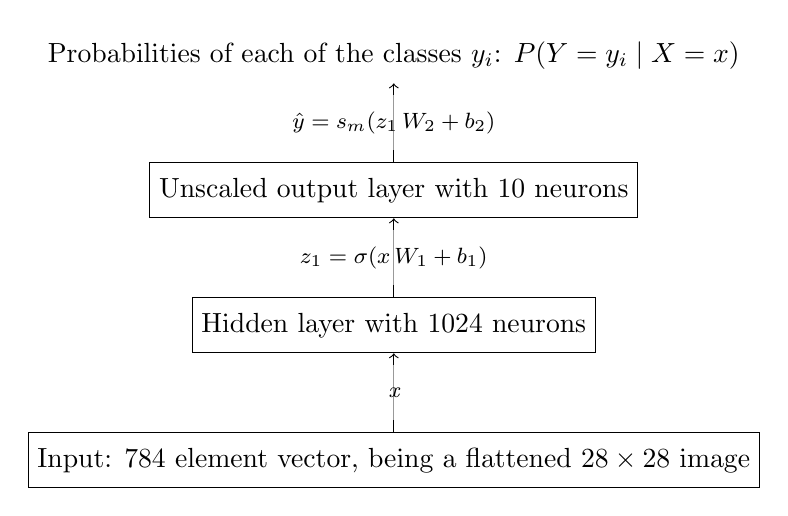
\begin{tikzpicture}[]

\node(in)[layer]{Input: 784 element vector, being a flattened $28 \times 28$ image};

\node(l1)[layer, above=of in]{Hidden layer with 1024 neurons};
\node(l2)[layer, above=of l1]{Unscaled output layer with 10 neurons};
\node(out)[above=of l2]{Probabilities of each of the classes $y_i$: $P(Y = y_i \mid X=x)$};

\draw[->] (in) edge  node[labe]{x} (l1);
\draw[->] (l1) edge  node[labe]{$z_1=\sigma(x\,W_1+b_1)$} (l2);
\draw[->] (l2) edge  node[labe]{$\hat{y}=s_m(z_1\,W_2+b_2)$} (out);

\end{tikzpicture}

\end{document}
\end{figure}

The network is defined by the equations:
\begin{align}
\v z&=\varphi(\d W_1 x + \dv b_1) \\
\hat{y}&=\softmax(\d W_2 z + \dv b_2) \\
P(Y{=}i{\mid}X{=}\v x) &= \hat{y}_i \\
&= \left[\softmax(\d W_2 \varphi(\d W_1 \v x + \dv b_1)+\dv b_2)\right]_i
\end{align}
for $X$ the input variable of grey-scale pixels intensities, and $Y$ the output as a class.
The output is represented with 1 hot encoding, where the index corresponding to the class is 1, and the others zero.


\aside[This simple network performs very well]{
	We note that this simple network can without further enhancement exceed the early published results for the MNIST challenge, using standard un-augmented neural networks,
	simply by using a very wide hidden-layer, that was not feasible at the time of those benchmarks.
	It is still outperformed by convolution neural networks and other better architectures.
}

To go into details about each layer:
The input is given by the grey scale pixel intensities in the original $28\times 28$ image.
This is flattened giving a $784$ element sized vector ($\v x$).
The first weight matrix projects that up onto a hidden layer  of width $1024$.
Thus $\d W_1$ is a $1024\times 784$ matrix.
The bias $\d {\v b}_1$ is for that hidden layer, so is a vector of length $1024$.
The hidden layer's actual activation values ($\v z$) for any input can be considered as being the values taken by 1024 different latent variables describing that input.
These are chosen  from a continuous abstract space of variables (via training) to effectively discriminate the correct class in the next layer (the output layer).

This is a shallow network, with only one hidden layer.
A deep network would have more hidden layers, for additional latent variables describing relations.
For the output layer we must project down to 10 dimensions, as there are 10 classes to choose from: the numbers from 0 to 9.
thus $\d W_2$ is a $10 \times 1024$ matrix,
and the bias $\dv b_2$ is a 10 element vector.
Using the softmax layer here ensures that output $\hat{y}$ is a valid probability mass function (nonnegative and summing to one).


\subsubsection{Softmax and Bayes' Theorem}\label{sec:softmax-and-bayes-theorem}
As a digression, it is worth considering the similarity between a network with a softmax output layer, and the application of Bayes' Theorem.
This will become important for understanding output embeddings, and hierarchical softmax in the future chapters.

The conditional probability of a classification given the value of some observed variable is defined by $P(Y=y\mid Z=\v z)$.
For $Y$ being the class taking value $i$;
and $Z$ the variable being conditioned upon, taking value $\v z$.
Here $\v z$  is some feature vector, this could be the output of a hidden layer below, or it could be a direct input.
Using softmax the estimated probability is given by
\begin{align} 
P(Y{=}i\mid Z{=}\v z) &= \i {\softmax(\v z)}_i\\
&=\frac{\exp{\i \left( W \v z+\v b\right)_{i}}}{\sum_{\forall j}\exp{\i \left( W \v z+\v b\right)_{j}}}\\
&=\frac{\exp{\i \left(W \v z \right)_{i}}\,\exp{\iv b_{i}}}{\sum_{\forall j}\exp{\i \left(W \v z\right)_{j}}\,\exp{\iv b_{j}}}
\end{align}

One can see that the bias term $\exp{\iv b_{i}}$ does not depend on the value of $z$.
The bias term is analogous to the prior probability.
Literally, it is the bias towards each element (i.e. each value $Y$ could take) without observing the condition.
We will define an unnormalised probability-like scoring function $R$;
and say $R(Y=i)=\exp{\iv b_{i}}$,
representing the marginal score contribution towards class $i$ from the bias.


The other component is $\exp{\i \left(W \v z \right)_{i}}$.
By considering this for each index $i$ (class value) that $Y$ might take then we have 
\begin{equation}
\i \left(W \v z \right)_{i}=\sum_{\forall j} \i W_{i,j} \, \iv z_{j} = \i W_{i,:} \v z
\end{equation}

Given one is considering the case for a particular class $Y=i$,
then it can be seen that the row vector $\i W_{i,:}$ as a weighting map for features possessed by $\v z$,
i.e. for input ($Z$) feature $j$, $\i W_{i,j}$ determines the relative weighting for that feature vs the other features of $Z$,
when the class is $i$.
When trained, the weight values should be such that it scores how likely the features are to occur for a given output class.
\pdfcomment{This sentence can be replaced wit ha stronger statement I think}

We can say that our scoring function $R$, has a likelihood term:
\begin{equation}
R(Z{=}\v z\mid Y{=}i)=\exp{\i \left(W \v z \right)_{i}}
\end{equation}

We will return to these row vectors  $\i W_{i,:}$ when we discuss as output embeddings in \Cref{sec:word-representations}.
$\i W_{i,:}$ must characterise the output class $i$, since difference classes would assign different importance to different features in the $Z$.
Furthermore, to some degree similar classes, i.e. classes triggered by similar features, would thus have more similar weights.


%
We can combine the unnormalised score factors to reformulate the original statement:
\begin{equation}
P(Y{=}i\mid Z{=}\v z)=\frac{R(Z{=}\v z\mid Y{=}i)\,R(Y{=}i)}{\sum_{\forall j}R(Z{=}\v z\mid Y{=}j)\,R(Y{=}j)}
\end{equation}


Contrast this to Bayes' Theorem:%
\aside[Marginal Denominator in Bayes Theorem]{In \Cref{eq:bayesmarginal}, notice that we replace $P(Z{=}\v z)$.
	We do this using the rule for finding marginal probabilities, from conditional probabilities with mutually exclusive and exhaustive condition values. This is always possible when working with classification.}%
%
\begin{align}
P(Y{=}i\mid Z{=}\v z)&=\frac{P(Z{=}\v z\mid Y{=}i)\,P(Y{=}i)}{P(Z{=}\v z)}\\
&=\frac{P(Z{=}\v z\mid Y{=}i)\,P(Y{=}i)}{\sum_{\forall j}P(Z{=}\v z\mid Y{=}j)\,P(Y{=}j)} \label{eq:bayesmarginal}
\end{align}



The similarities can be seen.
The bias effectively determines a prior probability-like term.
The weights defines the posterior probability: that is the chance of a particular class having a particular set of features.
The rows of the weight matrix mark how important each hidden feature is to each class. \pdfcomment{check rows vs cols}
We can consider that each row of the weight matrix is itself a representation of the class, as characterised by the importance of those latent features.
In the next chapter we will consider this as an output embedding.

A more traditional way of finding a representation of an input (rather than an output class) is to use an autoencoder.

\subsection{Bottlenecking Autoencoder}\label{sec:bottle-necking-autoencoder}

An autoencoder is a tool primarily used for finding a representation of their input.
There are many varieties of autoencoder based on neural network related techniques, including the works of \textcite{hinton2002RBM,hinton2006reducing,hinton2006fastDBN,vincent2010stacked,ICML2012Chen_416,2014VAE}.
This itself is a whole sub-field of machine learning.
Here we look at a simple bottlenecking autoencoder
\parencite{bourlard1988auto,japkowicz2000nonlinear}.
It has been used in a variety of tasks to attempt to find an optimal representation for an input e.g. as in \tcite{Usui:92}.
\begin{figure}
	\caption{A sampling of MNIST images from the test-set, arranged according to the values of 2 neurons on the encoding layer.}
	\label{mnist-encoding}
	\includegraphics[width=\textwidth]{figs/chapterintromachinelearning/mnist-encoding.png}
\end{figure}
An autoencoder is a neural network tasked with outputting its input.
This seemingly is a pointless task -- one already has the perfect reproduction of the input, in the input itself.
However, the true use of an autoencoder is to extract the output of one of the intermediary layers.
We call the intermediary layer the code layer.
To force this coded representation to have useful interesting properties,
and to prevent the network from simply learning the identity function,
all autoencoder include one or more features that increases the difficulty.
In the case of the bottlenecking autoencoder this feature is the bottleneck.
The code layer is much narrower than the input layer.
This forces the network to effectively learn to compress the data -- performing dimensionality reduction.

In this particular example we are looking at an auto-encoder for the MNIST images discussed earlier.
The original images are $28 \times 28$ pixels, i.e. 784 dimensional.
We compress it down to just 2 dimensions using the network shown in \Cref{fig-autoencoder}.

\begin{figure}
	\caption{A structure for a Bottle Necking Autoencoder for use on MNIST.}
	\label{fig-autoencoder}
	\resizebox{\textwidth}{!}{\documentclass{standalone}

\usepackage{tikz}
\usetikzlibrary{positioning, fit,  shapes.geometric}
\usepackage{ifthen}
\usepackage{etoolbox}

\tikzset{
	backgroundcolor/.style ={fill=white},
	every node/.append style={
		minimum height=7mm,
	},
	labe/.append style={
		%Blue,
		align = center,
		backgroundcolor,
		fill opacity=0.6,
		text opacity=1,
		font={\footnotesize\itshape}	
	},
	layer/.append style={
		draw,
		align = center,
		minimum height=7mm,
	},
	tight/.append style={
		inner sep=0.2mm,
	},
	lookupbox/.append style={
		draw=none,
		append after command={
		       	[shorten <= -0.5\pgflinewidth]
		       	([shift={(-1.5\pgflinewidth,-0.5\pgflinewidth)}]\tikzlastnode.north east)
		       	edge([shift={( 0.5\pgflinewidth,-0.5\pgflinewidth)}]\tikzlastnode.north west) 
		       	([shift={( 0.5\pgflinewidth,-0.5\pgflinewidth)}]\tikzlastnode.north west)
		       	edge([shift={( 0.5\pgflinewidth,-1.5\pgflinewidth)}]\tikzlastnode.south west)            
		       	([shift={( -1.5\pgflinewidth,+0.5\pgflinewidth)}]\tikzlastnode.south east)
		       	edge([shift={(-1.5\pgflinewidth,-0.5\pgflinewidth)}]\tikzlastnode.north east)
		},
		inner sep=0.7mm,
		outer sep=0mm,
		minimum width=25mm
	}
}

\begin{document}

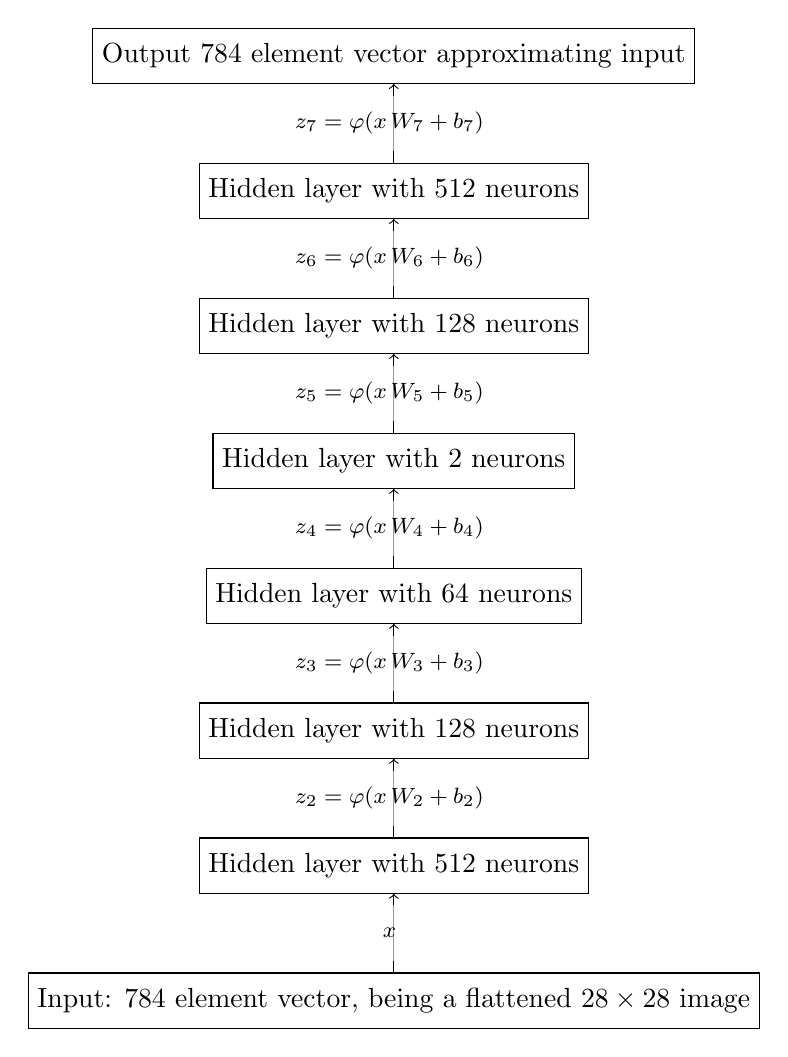
\begin{tikzpicture}[]

\node(L0)[layer]{Input: 784 element vector, being a flattened $28 \times 28$ image};

\foreach \i/\y[count=\j from 0] in {1/512, 2/128, 3/64, 4/2, 5/128, 6/512, 7/784}{
	\node(L\i)[layer, above= of L\j] {
		\ifthenelse{\j=6}{Output 784 element vector approximating input}%
		{Hidden layer with $\y$ neurons}%
	};
%
	\draw[->] (L\j) edge  node[labe]{
		\ifthenelse{\j = 0}{$x$}{$z_\i=\varphi(x\,W_\i+b_\i)$}
	}(L\i);	
}

%
\end{tikzpicture}

\end{document}}
\end{figure}

\FloatBarrier
In this particular network $\varphi$ is a leaky RELU6 unit.
\asidefig[The Leaky ReLU6 function. The leak level on this plot is exaggerated for purposes of visualisation.]{
	\begin{tikzpicture}
	\begin{axis}[sideplot,  xtick={-6, 0,6}, ytick={-3, 0,3,6}, enlarge y limits={abs=2}]
	\addplot+[equ] {max(0.05*x, min(1.05*x, 0.05*x + 6))};
	\end{axis}
	\end{tikzpicture}
}
\begin{equation}
\varphi(z)=\begin{cases}
    0.01z+6 & 6<z \\
	1.01z & 0 \le z \le 6 \\
	0.01z & z < 0
\end{cases}
\end{equation}

The reason for this is that a sigmoidal unit does not perform well in a deep network because of the gradient-vanishing/exploding effects.
As a result, only the bias information of the final layer mattered, effectively making all outputs just the average of all inputs.
The normal solution to this in deep networks is ReLU or ReLU6 units.

However, a ReLU, or ReLU6 unit is not ideal either,
as these units turn-off, and cannot turn back on again.
If one of the only 2 neurons in the code layer turn-off then they cannot turn back on again -- thus forcing it down to just one neuron, or none if that neuron also dies.
In trialling this network structure, this was found to occur quiet very often.

The solution was to add a ``leak'' to the unit.
A small constant gradient even in the saturated position.
Making such a neuron possible, even if difficult, to turn back on once turned off.
With this change the network always produces quality results.
An example of the recreation of an input from the test set can be seen in 
 \Cref{fig-ae-recreation}. 
It can be seen that the blur suggests that the input is a 7 or 9 like shape -- that level of information survived being squeezed through the bottleneck.


\asidefig[Recreation of an input from the MNIST test set. Input is on the left, output is on the right. 	{\label{fig-ae-recreation}}]{\includegraphics[scale=0.30]{figs/chapterintromachinelearning/recreation}}


More significantly, a sampling of the code layer is visually shown in \Cref{mnist-encoding}.
In this image, the positions on the X and Y axis for each input image is given by the values from the code layer for the representation of that image.
It can be seen that the code is capturing key information about the appearance.
The 0s appear near to the similarly rounded 6s,
the 8s near the 3s, etc.
In particular the 1s are arrayed according to their slope.
The autoencoder has captured very useful information about the inputs, that would be hard to define with any hand-written feature extractor.

It is this property of networks, to implicitly discover and define the most important latent variables and relationships to the task at hand that also makes it valuable for natural language processing.


\end{document}


\chapter{Current Challenges in Natural Language Processing}\label{sec:current-challenges-in-natural-language-processing}
\begin{abstract}
	Chapter 3: Current Challenges in Natural Language Processing (10 pages)
	Whereas chapter 2 introduces the Machine Learning domain, this chapter introduces the Natural Language Processing domain.
	This chapter will cover the current tasks that natural language processing is being deployed for
	It provide forward references to the works (in Part B) that use machine learnt representation to accomplish these tasks
	Particular tasks to be discussed include
	Language Modelling
	Sentiment Analysis
	Image Captioning
	Image generation
	Machine Translation
	Paraphrase and plagiarism detection
	Limited discussion will be presented here on prior, non-machine learning techniques.
\end{abstract}

%\part{Representations}\label{sec:representations}
%Part B: Representations

\documentclass[parskip]{komatufte}
\usepackage[subpreambles=false]{standalone}

%%%%%%%%%%%%%%%%%%%%%%%%%%%
% Silence warning messages
\usepackage{silence}
\WarningsOff[scrlayer-notecolumn]
\WarningsOff[biblatex]

%%%%%%%%%%%%%%%%%%%%
% Commenting

%\usepackage[author=Lyndon]{pdfcomment}
%\newcommand{\pdfcomment}[1]{} %ignore all comments

%\usepackage{todonotes}
%\newcommand{\pdfcomment}{\todo}


%%%%%%%%%%%%%%%%%%%%
% Tables
\usepackage{booktabs}

%%%%%%%%%%%%%%%%%%%
% Fonts
\usepackage{tgadventor} %sans
\usepackage{tgpagella}  %serif
\usepackage{inconsolata} %mono
\usepackage[T1]{fontenc}

\usepackage{microtype}
\usepackage[all]{nowidow}
%%%%%%%%%%%%%%%%%%%%%%%
% Styling
\setcounter{secnumdepth}{4}
\setcounter{tocdepth}{2}

\usepackage{placeins}



%%%%%%%%%%%%%%%%%%%
% Math
\usepackage{amsmath, amssymb, stmaryrd, mathtools}
\DeclareMathOperator*{\argmin}{argmin}
\DeclareMathOperator*{\argmax}{argmax}

\usepackage{xparse,xstring,etoolbox}
% crossref this against notation section
\newcommand{\vv}[1]{\tilde{#1}} % vector
\newcommand{\seq}[1]{\mathcal{#1}} % sequence
\newcommand{\set}[1]{\mathbb{#1}} % set

%%%%%%%%%
% Indexing/sequence indexing
\newcommand{\seqind}[2]{#1^{#2}} % seqence index
\newcommand{\ind}[2]{#1_{#2}} % indexed
\newcommand{\disamb}[2]{#1^{\mathrm{#2}}} %disambiguated

%% Smart indexing and naming
\newcommand{\ifupper}[3]{
    \normalexpandarg
	\exploregroups
	\StrCount{ABCDEFGHIJKLMNOPQRSTUVWXYZ}{#1}[\uppercount]
	\ifnumgreater{\uppercount}{0}{#2}{#3}
}

%smart index
\DeclareDocumentCommand{\ii}{u{_} m}{
	\ifupper{#1}%
	{% just a single uppercase character, i.e. a matrix
		  %make sure the index is the right length
		\StrCount{#2}{,}[\indcount]
		\ifnumgreater{\indcount}{0}
		{ % Got multiple indexes so all good
		 	\ind{#1}{#2}
		}
		{ % Only 1 index so grab the column
		 	\ind{#1}{{:,#2}}
		}
	}%
	{% Not just a single upper case character
		\ind{#1}{#2}
	}
}

\DeclareDocumentCommand{\nn}{u{_} m}{
	\seqind{#1}{#2}
}

\DeclareDocumentCommand{\dd}{u{_} m}{
	\disamb{#1}{#2}
}

% Index of a vector
\DeclareDocumentCommand{\iv}{u{_} m}{\ii{\vv #1}_{#2}}
\DeclareDocumentCommand{\dv}{u{_} m}{\dd{\vv #1}_{#2}}
\DeclareDocumentCommand{\nv}{u{_} m}{\nn{\vv #1}_{#2}}

%exp
\let\oldexp\exp
\renewcommand{\exp}[1]{\oldexp \left( #1 \right)}
\newcommand{\exptwo}[1]{\oldexp_2 \left( #1 \right)}

\newcommand{\softmax}{\mathrm{smax}}

\DeclareMathOperator*{\expectedop}{\mathbb{E}}
\DeclareDocumentCommand{\expected}{u{_} m}{
	\expectedop\limits_{\mathrlap{#2}}
}

%%%%%%%%%%%%%%%%
%Graphics
\usepackage{tikz}
\usetikzlibrary{positioning, fit,  shapes.geometric}
\usepackage{ifthen}
\usepackage{etoolbox}

\tikzset{
	backgroundcolor/.style ={fill=white},
	every node/.append style={
		minimum height=7mm,
	},
	labe/.append style={
		%Blue,
		align = center,
		backgroundcolor,
		fill opacity=0.6,
		text opacity=1,
		font={\footnotesize\itshape}	
	},
	layer/.append style={
		draw,
		align = center,
		minimum height=7mm,
	},
	tight/.append style={
		inner sep=0.2mm,
	},
	lookupbox/.append style={
		draw=none,
		append after command={
		       	[shorten <= -0.5\pgflinewidth]
		       	([shift={(-1.5\pgflinewidth,-0.5\pgflinewidth)}]\tikzlastnode.north east)
		       	edge([shift={( 0.5\pgflinewidth,-0.5\pgflinewidth)}]\tikzlastnode.north west) 
		       	([shift={( 0.5\pgflinewidth,-0.5\pgflinewidth)}]\tikzlastnode.north west)
		       	edge([shift={( 0.5\pgflinewidth,-1.5\pgflinewidth)}]\tikzlastnode.south west)            
		       	([shift={( -1.5\pgflinewidth,+0.5\pgflinewidth)}]\tikzlastnode.south east)
		       	edge([shift={(-1.5\pgflinewidth,-0.5\pgflinewidth)}]\tikzlastnode.north east)
		},
		inner sep=0.7mm,
		outer sep=0mm,
		minimum width=25mm
	}
}

\usepackage{pgfplots}
\pgfplotsset{compat=1.14}
\pgfplotsset{sideplot/.append style={
		width=\notescolwidth,
		domain=-10:10,
		samples=101,
		smooth,
		enlarge y limits={abs=2},
		axis lines=middle,
		xlabel  = $z$,
		ylabel  = $y$,
	},
	equ/.append style={
		color=blue,
		thick,
		mark=none
	}
}

% Function  For a plot 
% it  needs to be declared in preamble because of how \makenote* interacts with multiple files
\def\errorsurface(#1,#2){(0.5*#1 + 0.7*#2 + sin(deg(1.5*#1 + #2^2)))^2}


\usepackage{graphicx}
\graphicspath{{./figs/}, {./}, {./figs/chaptersentencerrepr/}, {./figs/chapterintromachinelearning/}, {./figs/chapterwordrepr/}}
\usepackage{adjustbox}


%%%%%%%%%%%%%%%%%%%
% Refs
\usepackage{cleveref}

\addbibresource{master.bib}

%%%%%%%%%%%%%%%%%%%%
% Formatting

% for examples from natural language space.
\newcommand{\natlang}[1]{\ifmmode \text{``\texttt{#1}''} \else {``\texttt{#1}''}\fi}
% \ifmmode ``trick'' from https://tex.stackexchange.com/a/15194/5834

%%%%%%%%%%%%%%%%%%%%%


\graphicspath{{./figs/chapterwordrepr}, {./}}


\begin{document}
\chapter{Word Representations}\label{sec:word-representations}
\begin{abstract}
The core work that began to draw a lot of attention to this area.
This will cover crucial works such as skip-grams, CBOW, and of course the original neural probabilistic language model.
As well as the links to traditional matrix factorisations.
\end{abstract}

\aside[Word Vector or Word Embedding?]{In some older literature in the area will use the term \emph{word~vector} to refer to representations from LDA and LSA etc. Whereas in a lot of newer work the term is used synonymously with \emph{word~embedding}.}
We begin the consideration of the representation of words using neural networks with work on language modeling
This is not the only place one could begin the consideration: the information retrieval (IR) models such as LSA \pcite{dumais1988using} and LDA \pcite{blei2003latent} based on word co-location with documents would be the other obvious starting point.
However, as will be discussed there models are closer to the end point of of the chapter than the begin.
For the language modeling works, comes the contextual language model works such as skip-gram, which in turn lead to the post-neural network co-occurrence based works.
These model fundamentally are in fact more similar to the information retrieval co-location works than the language modeling from which we began.


\section{Representations for Language Modeling}

\aside[Random Variable Naming Convention]{We follow convention that capitalised $W_i$ is a random variable, and $w_i$ is a particular value which $W_i$ may take. Writing $P(\ldots W_i{=}w_i)$.
	Often though we will make uses of the abridged (abuse-of) notation and simply write $P(\ldots w_i)$, allowing the random variable to be implicitly given by the name of its value.
}

The language modeling task it to predict the next word given the words that came prior \pcite{rosenfeld2000two}.
For example, if a sentence begins \natlang{For lunch I will have a hot}, then there is a high probability that the next word will be \natlang{dog} or \natlang{meal},
and lower probabilities of words such as \natlang{day} or \natlang{are}.
Mathematically it is formulated: 
\begin{equation}\label{equ:langmodel}
	P(W_n{=}w_i \mid W_{i-1}{=}w_{i-1}, \ldots, W_1{=}w_1)
\end{equation}
or to use the compact notation 
\begin{equation}\label{equ:langmodelcompact}
P(w_i \mid w_{i-1}, \ldots, w_1)
\end{equation}
$P(w_i \mid \natlang{hot}, \natlang{a}, \natlang{want}, \natlang{I}, \natlang{lunch}, \natlang{For})$.
The task is to find the probabilities for the various words that $w_i$ could represent.

\aside[Google n-gram corpora]{Google has created several very large scale corpora of 1,2,3,4, and 5-grams from over $10^{11}$ words.
Including the 2006 Web corpus from the public internet (Available for fees at \url{https://catalog.ldc.upenn.edu/LDC2006T13}),
and the 2010-2012 Books corpus made words from the Google Books project (available freely from \url{https://books.google.com/ngrams/datasets}), as described in \textcite{lin2012syntactic}.
These very large corpora also used outside of statistical language modeling by corpus linguists investigating the use of language.
}

  
The classical approach is trigram statistical language modeling.
In this, the number of word triples in a corpus is counted,
then given the previous two words, the next is predicted based on those counts.
This is making the Markov assumption that the next state depends only on the current state,
and that that state can be described by previous two words.
Under this assumption \Cref{equ:langmodelcompact} becomes:
\begin{equation}\label{equ:trigramlangmodel}
P(w_i \mid w_{i-1}, \ldots, w_1) = P(w_i \mid w_{i-1}, w_{i-2})
\end{equation}
More generally, one can use $n$-gram language model where for any value if $n$,
this is simply a matter of defining the Markov state to contain fewer or greater numbers of previous words than in the trigram case.

This Markov assumption is, of-course, an approximation.
In the previous example, a trigram language model is finding $P(w_i \mid \natlang{hot}, \natlang{a})$.
It can be seen that the approximation has lost key information.
Based only on the previous 2 words the next word $w_i$ could now reasonably be \natlang{day}, but the sentence: \natlang{For lunch I will have a hot day} makes no sense.
However, the Markov assumption in using $n$-grams is required in order to make the problem tractable -- otherwise an unbound amount of information would need to be stored. 

They key issue with n-gram language models in that in training them there is a data-sparsity problem.
Most combinations of words occur very rarely \pcite{ha2009extending}.
It is thus hard to estimate their occurrence probability.
Combinations of words that do not occur in the model is derived from as naturally given a probability of zero.
This is unlikely to be true though -- it is simply a matter of rare words never occurring together in a finite corpus.
Several approaches have been taken to handle this.
Simplest is add-one smoothing which adds an extra pseudo-observation of every combination of terms.
In common use is are various back-off methods \pcite{katz1987estimation,kneser1995improved} which use the bigram probabilities to estimate the probabilities of unseen trigrams.
%
\aside{An extended look at classical techniques in statistical language modelling can be found in \textcite{DBLP:journals/corr/cs-CL-0108005}}
%
However, these methods are merely clever statistical tricks -- ways to reassign probability mass after the fact to leave some left-over for unseen cases.
Back-off is smarter than add-one smoothing, as it portions the probability fairly based of the $n{-}1$-gram probability.
Better still would be a method which can learn to see the common-role of words.
By looking at the fragment: \natlang{For lunch I want a hot}, any reader knows that the next word is most likely going to be a food.
We know this for the same reason we know the next word in \natlang{For elevenses  I had a cold ...} is also going to be a food.
Even though \natlang{elevenses} is a vary rare word, we know from the context that it is a meal (more on this later), and we know it shares other traits with meals, and similarly \natlang{have} / \natlang{had}, and \natlang{hot} / \natlang{cold}.
These traits influence the words that can occur after them.
Thus the motivation is for a language modeling method that use these common properties of the words in the language modeling.
We need representation that holds this information.

\subsection{The Neural Probabilistic Language Model}

\tcite{NPLM} presents a method that uses neural network representations in a language model, where this representations implicitly learn the crucial traits of words.
Capturing the trait information in the representation of a word for use in language modeling is not an idea exclusive to neural network approaches.
Almost a decade earlier was the clustering work of  \tcite{brown1992class}.
The method of \tcite{NPLM} however, implicitly learns this information into a neural network bases representation in during the training for the language modeling task.

To understand the neural probabilistic language model, first consider a simplified neural trigram language model.
This model is a simplification of that introduces by \tcite{NPLM}, it forms the basis of several models and introduces the most important idea in neural language representations: that of training a vector representation of a word using a lookup table to map a discrete word to a vector that becomes the first layer of the network.



\aside[Lookup word embeddings: Hashmap or Array?]{
The question is purely one of implementation.
Theoretically we do not care if the implementation using a String to Vector dictionary (eg a Hashmap), or an 2D Array which is indexed into via an integer index representing the word, to retrieve a column.
In tokenization of the source text it is common to transform all the words into integers, so as to save memory, especially if the tokenization does not make use of string interning.
At that point it makes sense to work with a Array.
For our purposes we will treat the word $w_i$ as if it were an integer index, though thinking of it as a string index into a hashmap changes little in the logic.
}

\aside[One-hot product or Indexed-lookup]{
In some works you may see the process of retrieving the word vector from an Matrix of word vectors described as a one-hot multiplication.
That is to say for a word represented by the index $i$,
for $e_i$ the one-hot vector with a 1 in the $i$th position,
and for $C$ the table of word embeddings.
one can write  $C\,e_i$.
We will write $C_i$ and refer to this as looking up the word vector from the $i$th column.
Of-course $C_i=C\,e_i$, however in practical implementation the performance ramification are huge.
A matrix column indexing is a $O(1)$ operation (for column major languages),
where as a dense matrix-vector product is $O(n^2)$.
%
The one-hot product can be used in a pinch to support using embeddings in neural network toolkits that do not support lookup/embedding layers,
however we strongly suggest that if your toolkit does not support lookup/embedding layers then it is unsuitable for use in NLP applications.
}

The trigram neural probabilistic network is defined by:
%
\begin{multline}
P(w_i \mid w_{i-1}, w_{i-2}) = \\
s_{max}\left(V \: \varphi\left(U\left[C_{w_{i-1}}; C_{w_{i-2}}\right] + b_1\right)+b_2\right)
\end{multline}
%
where $U,\: V,\: b_1,\: b_2$ are the weight matrices and biases of the network, and $C_{w_{i-1}}$ and $C_{w_{i-2}}$ are the looked-up word embedding for the previous two words, from the embedding table $C$.
We write $\left[v_1; v_2\right]$ as a notational convenience for the concatenation of vectors $v_1$ and $v_2$.
The network is shown diagrammatically in \Cref{fig:trigram-neural-language-model}

\begin{figure}
	\centering
	\documentclass{article}

\usepackage{tikz}
\usetikzlibrary{positioning, fit,  shapes.geometric}
\usepackage{ifthen}
\usepackage{etoolbox}

\tikzset{
	backgroundcolor/.style ={fill=white},
	every node/.append style={
		minimum height=7mm,
	},
	labe/.append style={
		%Blue,
		align = center,
		backgroundcolor,
		fill opacity=0.6,
		text opacity=1,
		font={\footnotesize\itshape}	
	},
	layer/.append style={
		draw,
		align = center,
		minimum height=7mm,
	},
	tight/.append style={
		inner sep=0.2mm,
	},
	lookupbox/.append style={
		draw=none,
		append after command={
		       	[shorten <= -0.5\pgflinewidth]
		       	([shift={(-1.5\pgflinewidth,-0.5\pgflinewidth)}]\tikzlastnode.north east)
		       	edge([shift={( 0.5\pgflinewidth,-0.5\pgflinewidth)}]\tikzlastnode.north west) 
		       	([shift={( 0.5\pgflinewidth,-0.5\pgflinewidth)}]\tikzlastnode.north west)
		       	edge([shift={( 0.5\pgflinewidth,-1.5\pgflinewidth)}]\tikzlastnode.south west)            
		       	([shift={( -1.5\pgflinewidth,+0.5\pgflinewidth)}]\tikzlastnode.south east)
		       	edge([shift={(-1.5\pgflinewidth,-0.5\pgflinewidth)}]\tikzlastnode.north east)
		},
		inner sep=0.7mm,
		outer sep=0mm,
		minimum width=25mm
	}
}

\begin{document}

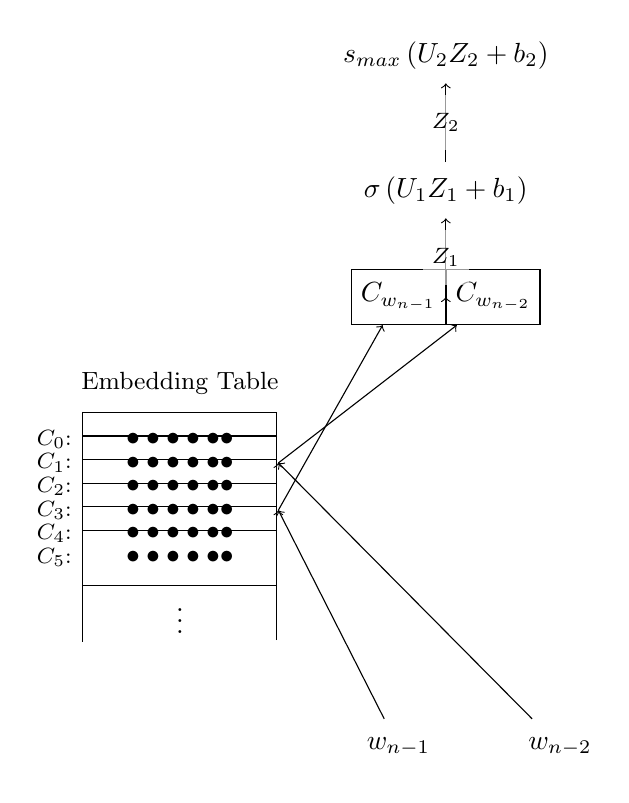
\begin{tikzpicture}[]


\node(w1) {$w_{n-1}$};
\node(w2)[right = of w1] {$w_{n-2}$};


\node(Cn)[lookupbox, above left=of w1] {$\vdots$};
\def\tblmax{6}
\foreach \ii in {1,...,\tblmax} {
	\pgfmathsetmacro\pos{(\ii - 1) * 3 };
	\pgfmathtruncatemacro\jj{(\tblmax -\ii)};
	
	\node(C\ii)[lookupbox, above = \pos mm of Cn]{$\bullet\bullet\bullet\bullet\bullet\bullet$};
	\node(Clbl\ii)[left = 0mm of C\ii]{\footnotesize $C_\jj$:};
};
\node(C)[above = 0mm of C\tblmax] {\small Embedding Table};



\node(concat1)[layer, above = 5 of w1]{$C_{w_{n-1}}$};
\node(concat2)[layer, right = 0 of concat1]{$C_{w_{n-2}}$};

\draw[->] (w1) edge (C3.east);
\draw[->]  (C3.east) edge (concat1);
\draw[->] (w2) edge (C5.east);
\draw[->]  (C5.east) edge (concat2);

\node(L1)[above = of concat1.east]{$\sigma\left(U_1Z_1 + b_1\right)$};
\draw[->]  (concat1.east) edge node[labe]{$Z_1$} (L1);

\node(L2)[above = of L1]{$s_{max}\left(U_2 Z_2 + b_2\right)$};
\draw[->]  (L1) edge node[labe]{$Z_2$} (L2);

\end{tikzpicture}

\end{document} 
	\caption{\label{fig:trigram-neural-language-model} Neural Trigram Language Model}
\end{figure}

In the neural trigram language model, each of the previous two words is used to look-up a vector from the Embedding Table matrix.
These are then concatenated to give a dense, continuous-space input to the above hidden layer.
The output layer is a softmax layer, it gives the probabilities for each word in the vocabulary, one of which corresponds to $w_i$ the word being evaluated.

The word embeddings are trained, via the normal neural network method, along with the network weights and biases.
This allows the embeddings of words which predict the same future word to move to be near each other in vector space.
It also allows the hidden layer to learn to associate information with regions of the embedding space.
This thus allows for information sharing between words.
If two words vectors are close together because they mostly predict the same future words, then that area of space is a associated with predicting those words.
Thus for cases where there are some words which never co-occur in the training set, but for which the nearby word does co-occur with, then because the knowledge is associated with that region of space, the model predicts that there is a higher-than-zero chance of the first word co-occurring with the unseen word.
This is a fuzzy and nonlinear relationship, with varying degrees of closeness resulting in (and from) varying levels of exception of the words sharing co-occurring predicted words.


\tcite{NPLM} is a more advanced version of the neural language model discussed.
Rather than being a trigram language model, it is an $n$-gram language model, where $n$ is a hyper-parameter of the model.
The knowledge sharing allows the data-sparsity issues to be ameliorated, thus allowing for $n>3$.
%
\aside{\textcite{schwenk2004efficient} suggests using only a subset of the vocabulary as options for the output, while allowing the full vocabulary in the input space -- with a fallback to classical language models for the missed words.
	This decreases the size of the softmax output layer, substantially decreasing the network evaluation and training time.
	This technique is now largely eclipsed by hierarchical softmax etc. discussed later in this chapter.
}
%
Bengio et. al. investigates values for $n$ of 3, 5 and 6.
The network used in their work also was marginally more complex, as shown in \Cref{fig:neural-language-model} and in the following equation:
\begin{align}
P(w_i & \mid w_{i-1}, w_{i-2}) = s_{max}( \nonumber
\\  & \quad U_3 \left[ C_{w_{i-1}};...; C_{w_{i-n}}\right] \nonumber
\\  & + V \: \varphi\left( U\left[C_{w_{i-1}};...; C_{w_{i-n}} \right] + b_1\right) \nonumber
\\  & +b_2)
\end{align}

It includes a layer-bypass, which is primarily present only as connivance to aid in the learning.
It allowing the input to directly effect the output without being mediated by the shared hidden layer.
This layer-bypass is a unusual feature, not present in future works deriving from this, such as \tcite{schwenk2004efficient} which presents a bag of tricks to minimize training time. 





This is the network which begins the notions of using neural networks with vector representations of words.
Bengio et. al. focused on the use of the of sliding window of previous words -- much like the traditional n-grams.
At each time-step the window is advanced forward and the next word predicted based on that shifted context of prior words.
They do very briefly mention that an RNN could be used in its place.

\begin{figure}
	\centering
	\documentclass{article}

\usepackage{tikz}
\usetikzlibrary{positioning, fit,  shapes.geometric}
\usepackage{ifthen}
\usepackage{etoolbox}

\tikzset{
	backgroundcolor/.style ={fill=white},
	every node/.append style={
		minimum height=7mm,
	},
	labe/.append style={
		%Blue,
		align = center,
		backgroundcolor,
		fill opacity=0.6,
		text opacity=1,
		font={\footnotesize\itshape}	
	},
	layer/.append style={
		draw,
		align = center,
		minimum height=7mm,
	},
	tight/.append style={
		inner sep=0.2mm,
	},
	lookupbox/.append style={
		draw=none,
		append after command={
		       	[shorten <= -0.5\pgflinewidth]
		       	([shift={(-1.5\pgflinewidth,-0.5\pgflinewidth)}]\tikzlastnode.north east)
		       	edge([shift={( 0.5\pgflinewidth,-0.5\pgflinewidth)}]\tikzlastnode.north west) 
		       	([shift={( 0.5\pgflinewidth,-0.5\pgflinewidth)}]\tikzlastnode.north west)
		       	edge([shift={( 0.5\pgflinewidth,-1.5\pgflinewidth)}]\tikzlastnode.south west)            
		       	([shift={( -1.5\pgflinewidth,+0.5\pgflinewidth)}]\tikzlastnode.south east)
		       	edge([shift={(-1.5\pgflinewidth,-0.5\pgflinewidth)}]\tikzlastnode.north east)
		},
		inner sep=0.7mm,
		outer sep=0mm,
		minimum width=25mm
	}
}

\begin{document}

\begin{tikzpicture}[]


\node(w1) {$\n w_{i-1}$};
\node(w2)[right = 0mm  of w1] {$\n w_{i-2}$};
\node(w3)[right = 0mm of w2] {$\ldots$};
\node(w4)[right = 0mm of w3] {$\n w_{i-n}$};


\node(Cn)[lookupbox, above left=of w1] {$\vdots$};
\def\tblmax{6}
\foreach \ii in {1,...,\tblmax} {
	\pgfmathsetmacro\pos{(\ii - 1) * 3 };
	\pgfmathtruncatemacro\jj{(\tblmax -\ii)};
	
	\node(C\ii)[lookupbox, above = \pos mm of Cn]{$\bullet\bullet\bullet\bullet\bullet\bullet$};
	\node(Clbl\ii)[left = 0mm of C\ii]{\footnotesize $\i C_\jj$:};
};
\node(C)[above = 0mm of C\tblmax] {\small \textsc{Embedding Table}};


\node(concat1)[layer, above = 5 of w1]{$\i C_{\n w_{i-1}}$};
\node(concat2)[layer, right = 0 of concat1]{$\i C_{\n w_{i-2}}$};
\node(concat3)[layer, right = 0 of concat2]{$\quad\ldots\quad$};
\node(concat4)[layer, right = 0 of concat3]{$\i C_{\n w_{i-n}}$};
 
\draw[->] (w1) edge (C3.east);
\draw[->]  (C3.east) edge (concat1.south);
\draw[->] (w2) edge (C5.east);
\draw[->]  (C5.east) edge (concat2.south);
\draw[->] (w4) edge (C5.east);
\draw[->]  (C5.east) edge (concat4.south);

\node(L1)[layer, above = of concat2.north east]{$\varphi\left(\d U_{hid}\dv z_{embs} + \v b\right)$};
\draw[->]  (concat2.north east) -- node[labe]{$\dv z_{embs}$} (L1);


\node(L2)[layer, above = of L1]{$s_{max}\left(V \dv z_{hid} +\d U_{bypass} \dv z_{embs}+ \v k\right)$};
\draw[->]  (L1) edge node[labe]{$\dv z_{hid}$} (L2); 
\draw[->, bend right] (concat2.north east)  to[bend right=45, min distance=25 mm] (L2);


\node(out)[above = of L2]{$P(\n w_i \mid \n w_{i-1}, \n w_{i-2}, \ldots, \n w_{i-n})$};
\draw[->] (L2) edge (out);


\end{tikzpicture}

\end{document} 
	\caption{\label{fig:neural-language-model} Neural Probabilistic Language Model}
\end{figure}


\subsection{RNN Language Models}

\aside[Differences in formulation]{
The network and equations shown here may seem different to those presented in \textcite{mikolov2010recurrent}.
However they are mathematically identical.
The apparent difference is simply the choice between considering embeddings as a look-up, or as a one-hot multiplication.
}

In \tcite{mikolov2010recurrent} an RNN is for a language model.
To be precise, an Elman network is used \tcite(elman1990finding).
In this form of RNN, the output of hidden layer in the previous time-step is appended as an additional input.
Using an RNN eliminates the sliding window of earlier language models.
Instead, the context information is stored in the state that is passed forward.

This state $Z_{j}$ being the hidden state output from the first (only) hidden layer when input the $j$th word, 
is given by 

\begin{equation}
	Z_{j} = \varphi\left( U\,Z_{j-1} + C_{w_{i-1}} \right)
\end{equation}


This hidden layer was the an input to the hidden-layer at the next time-step, as well as to the output softmax.

\begin{equation}
	P(w_i \mid w_{i-1}, ... w_{1}) = s_{max}\left(V \, Z_{i-1} \right)
\end{equation}



Rather than using an Elman network, a more advanced RNN such as Long-Short-Term-Memory (LSTM), or a Gated Recurrent Unit (GRU) \pcite{cho2014properties}, based network could be used.
The structure would remain very similar,
and additional advantages may be found from the improved stability and performance.

\tcite{sundermeyer2012lstm} investigated using LSTM.
This did indeed offer an improvement over the Elman network used in \textcite{mikolov2010recurrent}.
\tcite{jozefowicz2015empirical} conducted an extensive search of hyper-parameters for LSTM and GRU networks for language modeling.
For the best performing networks of both types the results found were significantly better than \textcite{sundermeyer2012lstm} and \textcite{mikolov2010recurrent}.
They found the best was the LSTM network, particularly if the forget gate was biased to a 1.0 or more.

\begin{figure}
	\centering
	\documentclass{article}

\usepackage{tikz}
\usetikzlibrary{positioning, fit,  shapes.geometric}
\usepackage{ifthen}
\usepackage{etoolbox}

\tikzset{
	backgroundcolor/.style ={fill=white},
	every node/.append style={
		minimum height=7mm,
	},
	labe/.append style={
		%Blue,
		align = center,
		backgroundcolor,
		fill opacity=0.6,
		text opacity=1,
		font={\footnotesize\itshape}	
	},
	layer/.append style={
		draw,
		align = center,
		minimum height=7mm,
	},
	tight/.append style={
		inner sep=0.2mm,
	},
	lookupbox/.append style={
		draw=none,
		append after command={
		       	[shorten <= -0.5\pgflinewidth]
		       	([shift={(-1.5\pgflinewidth,-0.5\pgflinewidth)}]\tikzlastnode.north east)
		       	edge([shift={( 0.5\pgflinewidth,-0.5\pgflinewidth)}]\tikzlastnode.north west) 
		       	([shift={( 0.5\pgflinewidth,-0.5\pgflinewidth)}]\tikzlastnode.north west)
		       	edge([shift={( 0.5\pgflinewidth,-1.5\pgflinewidth)}]\tikzlastnode.south west)            
		       	([shift={( -1.5\pgflinewidth,+0.5\pgflinewidth)}]\tikzlastnode.south east)
		       	edge([shift={(-1.5\pgflinewidth,-0.5\pgflinewidth)}]\tikzlastnode.north east)
		},
		inner sep=0.7mm,
		outer sep=0mm,
		minimum width=25mm
	}
}

\begin{document}

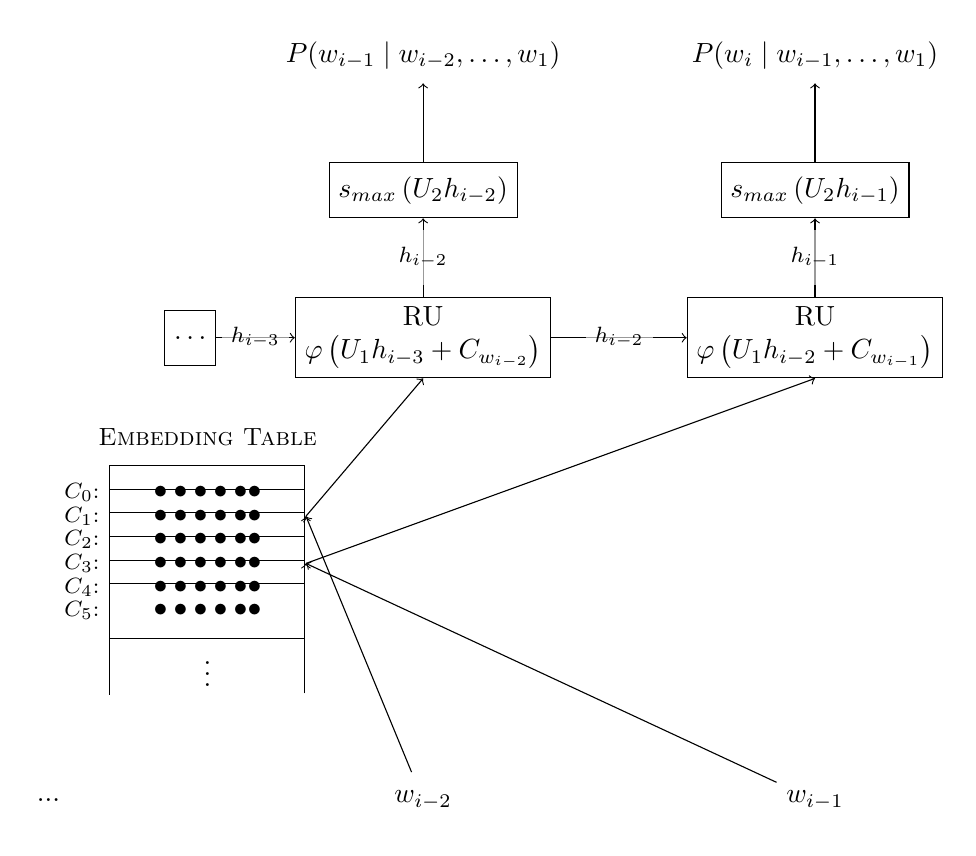
\begin{tikzpicture}[]

\newcommand{\hsep}{4}
\newcommand{\vtablesep}{5}

\node(w1) {$w_{i-1}$};
\node(w2)[left = \hsep of w1] {$w_{i-2}$};
\node(w3)[left = \hsep of w2] {$...$};


\node(Cn)[lookupbox, above left=of w2] {$\vdots$};
\def\tblmax{6}
\foreach \ii in {1,...,\tblmax} {
	\pgfmathsetmacro\pos{(\ii - 1) * 3 };
	\pgfmathtruncatemacro\jj{(\tblmax -\ii)};
	
	\node(C\ii)[lookupbox, above = \pos mm of Cn]{$\bullet\bullet\bullet\bullet\bullet\bullet$};
	\node(Clbl\ii)[left = 0mm of C\ii]{\footnotesize $C_\jj$:};
};
\node(C)[above = 0mm of C\tblmax] {\small \textsc{Embedding Table}};

\node(L11)[layer, above = \vtablesep of w1]{RU\\$\varphi\left( U_1h_{i-2}  +  C_{w_{i-1}}\right)$};
\node(L21)[layer, above = of L11]{$s_{max}\left(U_2 h_{i-1}\right)$};
\draw[->]  (L11) edge node[labe]{$h_{i-1}$} (L21);
\node(out1)[above = of L21]{$P(w_i \mid w_{i-1}, \ldots,  w_1)$};
\draw[->] (L21) edge (out1);

\node(L12)[layer, above = \vtablesep of w2]{RU\\$\varphi\left( U_1h_{i-3}  +  C_{w_{i-2}}\right)$};
\node(L22)[layer, above = of L12]{$s_{max}\left(U_2 h_{i-2} \right)$};
\draw[->]  (L12) edge node[labe]{$h_{i-2}$} (L22);
\node(out2)[above = of L22]{$P(w_{i-1} \mid w_{i-2}, \ldots,  w_1)$};
\draw[->] (L22) edge (out2);
\draw[->]  (L12) edge node[labe]{$h_{i-2}$} (L11);

\node(L13)[layer, left = of L12] {$\ldots$};
\draw[->]  (L13) edge node[labe]{$h_{i-3}$} (L12);


\draw[->] (w1) edge (C3.east);
\draw[->]  (C3.east) edge (L11.south);
\draw[->] (w2) edge (C5.east);
\draw[->]  (C5.east) edge (L12.south);


\end{tikzpicture}

\end{document} 
	\caption{\label{fig:neural-language-model} RNN Language Model}
\end{figure}

This ends our discussion of standard language models.


\section{Acausal Language Modeling}
The step beyond a normal language model,
which uses the prior words to predict the next word,
is what we will term acausal language modelling.
Here we use the word acausal in the signal processing sense.
The task here is to predict a missing word, using the words the preceed it, as well as the words that come after it.

As it is acausal it can not be done in a real-time system, and is not useful for many tasks directly.
However, what it is very useful for is as a task to learn a good representation for words.


\subsection{Context RNN}


\aside[Are CBOW \& Skip-Gram Neural Networks]{As these models do not have any non-linearities  (some would say they have no hidden layer, though is is incorrect: the projection layer of the embedding is functionally a hidden layer) it may be asserted that they are not in-fact neural networks at all.
This distinction is purely academic though.
Any toolkit that can well handle the prior discussed neural network models, can be very well used to implement CBOW and Skip-Gram.
}


\pdfcomment{I think CBOW and Skip-Gram don't feature Biases because they are written in Design Matrix form with a column of ones. If so I need to fix that up to something consistent with the remainder of this chapter or if not then }

\subsection{CBOW}
The continuous bag of words (CBOW) method was introduced by \tcite{mikolov2013efficient}.
In truth this is not particularly similar to bag of words at all, no more so than any other word representation that does not have regard for order of the context words (e.g. skip-gram, GloVE below).


For a context window of width $n$ words -- i.e. $\frac{n}{2}$ words to either side, of the target word,
the CBOW model is defined by:
\begin{align}
P(w_i & \mid w_{i-\frac{n}{2}},..., w_{i-1}, w_{i+1},...,w_{i+\frac{n}{2}})  \nonumber
\\  & = s_{max}(U \sum_{j=i+1}^{j=\frac{n}{2}} \left( C_{w_{i-j}}+C_{w_{i+j}} \right))
\end{align}

\pdfcomment{Need to consider that this is always done with a Hierarchical softmax, and check this formulation is correct}


\tcite{mikolovSkip}

\subsection{Skip-gram}
\tcite{mikolovSkip}

\aside[Skip-gram naming]{In different publications this model may be called skipgram skip-gram, skip-ngram, skip-gram etc. Further, it may be called \texttt{word2vec} after the publicly released implementation of the algorithm. Though that software also can be used for CBOW.}


The converse of CBOW is the skip-grams model \tcite{mikolov2013efficient}.
In this model, the central word is used to predict the words in the context.
While in CBOW each training case of context and target word presents one correct answer,
in the Skip-gram each training case has a number of correct answers, the probability of all of which in the softmax must be increased.

\begin{equation}
P(w_j \mid w_{i}) = \left[ s_{max}(V\,C_{w_{i}}) \right]_{w_j} 
\end{equation}


The goal, is to maximise the probabilities of all the observed outputs from the window's in the training set ($i-\frac{n}{2},...,i-1, i+i,...,i+\frac{n}{2}$).


This can be done using softmax, or hierarchical softmax (as in CBOW and other models).
Or an alternative option is suggested, negative sampling.

Note that Skip-Grams only hidden layer is the embedding layer.
If we take the earlier discussed notion of considering the output matrix $V$ as being an embedding layer/
This becomes:

\begin{align}
P(w_j \mid w_{i}) & = \left[ s_{max}(V\,C_{w_{i}}) \right]_{w_j} \\
P(w_j \mid w_{i}) & = \frac{\exp(V_{w_j}^\prime\,C_{w_{i}})}{\sum_{k=1}^{k=N} \exp(V_k^\prime\,C_{k})}
\end{align}

The key term here is the $V_{w_j}^\prime\,C_{w_{i}}$,
the remainder of the expression is normalising this into a probability.
Maximising the probability $P(w_j \mid w_{i})$ is equivalent to maximising the dot produce between $V_{w_j}^\prime$, the output embedding for $w_j$ and  $C_{w_i}$ the input embedding for $w_i$.
Which is to say that the skip-gram probability is maximises when the angular difference between the input embedding for a word, and the output embeddings for words that it co-occurs with is minimised, and the embeddings themselves are maximised.
\pdfcomment{Does maximising the embedding cancel out?}.


While skip-gram and CBOW were introduces in the same set of papers, subsequent work has found the skip-gram is almost always the preferred system for any task. \pdfcomment{Citation for this?}

\subsection{Analogy Tasks}
\aside[Using Analogy Tasks to discover subtle prejudice in corpora]{
}

It is on these systems that evaluation the analogy tasks became well known, though they were considered earlier on RNN neural language models \pcite{mikolov2013linguisticsubstructures}.
These tasks are keyed around answering the question: What is  \emph{c} and \emph{b} is to \emph{a}.
For example, a semantic analogy would be answering that \natlang{Aunt} is to \natlang{Uncle} as \natlang{King} is to \natlang{Queen}.
For example, a syntactic analogy would be answering that \natlang{Kings} is to \natlang{King} as \natlang{Queens} is to \natlang{Queen}.
The latest and largest analogy test set is presented by \tcite{gladkova2016analogy},
which evaluates embedding on 40 subcategories of knowledge.

The analogies work by relating similarities of offsets.
Word Similarity can be evaluated using word embeddings using a number of metrics.
By far the cosine similarity is the most common.
This is given by $sim(C_u, C_v)=\frac{C_{u}\cdot C_{v}}{\left\Vert u\right\Vert \left\Vert v\right\Vert }$.
A smaller distance in vector space, means the words are more similar -- in some sense.
Depending on the system this similarity could be syntactic, semantic or otherwise, the analogy tasks can help identify what kinds of similarities the embeddings are capturing.

Using the similarity scores a ranking of words to complete the analogy is found.
To find the correct word for \emph{d} in \emph{d} is to \emph{c} and \emph{b} is to \emph{a}
the following is computed for the table of embeddings $C$:
\begin{equation}
\argmax_{\forall d} sim(C_d, C_a-C_b+C_c)
\end{equation}

\pdfcomment{Insert Vector diagram here it will clarify reason for the math}

Initial results were relatively poor, but the surprising finding was that this worked at all. \pdfcomment{Citations here}.
Subsequent results found in \tcite{pennington2014glove} were much better.

\section{Co-location Factorisation}

\subsection{GloVe}

Skip-grams are intrinsically prediction based methods, effectively predicting what words will co-occur in the context of a local window and optimising as such.
In \tcite{pennington2014glove}the authors show that if one were to change that optimisation to be global over all co-occurrences,
then the optimisation critia becomes minimising the cross-entropy between the true co-occurrence probabilities given by $P(w_j\mid w_j)$, and the value of the embedding product: the cross entropy measure.,
weighted by the frequency of the occurrence of the word $X_i$.
That is to say if skip-gram were optimised globally it would be equivalent to minimising:
\begin{equation}
J = - \sum_{\forall w_i} \sum_{\forall w_j} X_{ij} P(w_j\mid w_j) \log (V_{w_j}^\prime\,C_{w_{i}})
\end{equation}

Minimising this cross-entropy efficiently means factorising the true co-occurrence matrix,
into the input and output embedding matrices $C$ and $V$, under a particular set of weightings given by the cross entropy measure.

\tcite{pennington2014glove} consider instead factorizing the logarithm of co-occurrence matrix directly,
the logarithm giving an different, but similar, weighting to the cross entropy measure.
Thas is for each word co-occurrence of $w_i$ and $w_j$: Attempting to find optimal values for 
the embeddings $C_{w_{i}}$, and $V_{w_j}^\prime$, while also allowing constant offsets $b_i$ and $k_j$
such that:
$V_{w_j}^\prime\,C_{w_{i}} + b_i + k_j \approx \log(X_{ij})$
as near as is possible.

\aside[Implementing GloVe]{To implement GloVe in any technical programming language with good support for matrix factorisation via least-squares optimisation is trivial. As is implementing any other matrix factorisation/dimensionality reduction based method.}

The precise measure used to do this, is a weighted the least squares minimisation of 
\begin{equation}
J = - \sum_{\forall w_i}  \sum_{\forall w_j} f(X_{ij})\,V_{w_j}^\prime\,C_{w_{i}}+b_i+k_j-\log (X_ij)
\end{equation}


using the weighting between 0 and 1 given by $f(x)$
\begin{equation}
f(x)=\begin{cases}
\left(\frac{x}{100}\right)^{0.75} & x<100\\
1 & otherwise
\end{cases}
\end{equation}
though they suggest other weightings may be suitable.
This can be contrasted as a saturating variant of the effective weighing of skip-gram being $X_{ij}$.
Though the variation in measure away from cross-entropy also significant and has related effects on the weightings of rare vs common words in the minimisation.

While in initial tests it was found that Glove out-performed  skip-gram,
subsequent more extensive testing in \tcite(levy2015) with more tuned parameters,
found that skip-gram out-performed GloVE on all tasks, though the performance is relatively comparable.



\aside[Key Factors Mentioned as Minor Tweaks]{
There is an interesting pattern of important factors being considered as not part of the core algorithm.
GloVe explicitly weights all co-occurrences inversely by the distance from each other -- though this is considered part of finding the co-occurrence matrix rather than part of the algorithm itself.
Skip-Gram accomplishes something similar with dynamic window sizing tweak -- the true size of the window is uniformly distributed between 1 and the value given.

GloVe explicitly scales the weight of terms to be optimised -- using the weighting function, which saturates for frequent terms.
Skip-Gram accomplishing something similar again using the sub-sampling tweak -- common words are randomly skipped from the contexts during training, based on how common they are.

While the authors papers consider these as unimportant to the main thrust of the algorithms \textcite{levy2015} found them to be crucial hyper-parameters.
}

However, GloVe loosely highlights the relationship between the co-located word prediction neural network models,
and the more traditional matrix factorization of collocation counts used in topic modeling.
Very similar properties were also explored for skip-grams with negative sampling in \tcite{levy2014neural} and then in \tcite{li2015wordemedingasEMF} with more direct mathematical equivalence to weighed co-occurrence matrix factorisation;
Later in \tcite{cotterell2017SkipgramisEPCA} showed the equivalence to exponential principal component analysis also.



\subsection{Conclusion}
As we have now concluded that neural predictive co-location models are functionally very similar to matrix factorisation of co-location counts with suitable weightings, and suitable similarity metrics.
One might suggest a variety of word embeddings to be created from a variety of different matrix factorisations with different weightings and constraints; and indeed this has been done.
Traditionally large matrix factorisations have significant problems in terms of computational time and memory complexity.
A common solution to this is to handle it an iterative optimisation procedure.
Training a neural network such as skip-gram is an iterative optimisation procedure.











\section{Natural Language Applications -- beyond language modeling}
While statistical language models are useful, they are of-course in no way the be-all and end-all of natural language processing.
Simultaneously with the developments around representations for the language modelling tasks, work was being done on solving other NLP problems using similar techniques.

\tcite{collobert2008unified}


\subsection{Using Word Embeddings as Features}

\aside[Pretrained Word-Embeddings]{
	Pretrained Word Embeddings are available for most models discussed here.
	There trained on a lot more data than most people have access too.
	It can be useful to substitute word embeddings are a representation in most systems,
	or to use them as intitial value for neural network systems that will learn them as they train the system as a whole.
\pdfcomment{Insert links}
}

\tcite{turian2010word} discusses what is now perhaps the most important use of word embeddings.
The use of the embeddings as features, in unrelated feature driven models.
One can find word embeddings using any of the methods discussed above, for example language modelling.
These embeddings can be then used as features instead of, for example bag of words or hand-crafted feature sets.
\tcite{turian2010word} found improvements on the state of the art for chunking and Named Entity Recognition (NER), using the word embedding methods of that time.
Since then, these results have been superseded again using newer methods.



\section{Aligning Vector Spaces Across Languages}
Given two vocabulary vector spaces, for example one for German and one for English,
a natural and common question is if they can aligned such that one has a single vector space for both.
Using canonical correlation analysis (CCA) one can do exactly that.
Here, we will discuss normal CCA for aligning two vectors spaces,
though there also exists generalised CCA for any number of vector spaces \pcite{gcca}.

The inputs to CCA, are two sets of vectors, normally expressed as matrices,
Which we will call for consistency $C \subseteq \mathbb{R}^{n_1}$ and $V \subseteq \mathbb{R}^{n_2}$.
These are both some set of vector representations for words, not necessarily of same dimensionality.
These could be the output of any of the embeddings dicusses earlier,
or even a sparse (non-embedding) representations such as the point-wise mutual information of the co-occurrence counts.
The other input is an a subset of pairs from those sets that are to be aligned, which we will call, $C^\star \times V^\star$.
This subset contains only pairs with known translations -- this does not have to be the whole vocabulary of either language.


%
By performing CCA (the details of which are well out of scope for this text),
one solves to find a series of vectors, $S=\left[ \tilde{s}_1, ..., \tilde{s}_d \right]$ and $T= \left[ \tilde{t}_1, ..., \tilde{t}_d\ \right]$,
such that the correlation between $\tilde{s}_i^\prime C^\star$ and $\tilde{t}_i^\prime V^\star$ is maximised,
while constraining with the requirement for all $j<i$ that $\tilde{s}_i^\prime C^\star$ is uncorrelated with $\tilde{s}_j^\prime C^\star$  and that  $\tilde{t}_i^\prime V^\star$ is uncorrelated with $\tilde{t}_j^\prime V^\star$.
This is very similar to principal component analysis(PCA), and like PCA number components to use $d$ is a variable that can be deceased to achieve dimensionality reduction.
When complete, taking $S^\prime$ and $T^\prime$ as matrices gives projection matrixes that project $C$ and $V$ to a space where aligned elements are as correlated as possible.
That is to say the final new common vector space embeddings are given by:
$S^\prime C$ and $T^\prime V$.
\pdfcomment{Check this, both for correctness in decription, and for correctness in notation.}

\textcite{faruqui2014improving} investigated this primarily as a means to use additional data to improve performance on monoligual tasks.
In this they found small and inconsistent improvement.
However
However, we suggest it is much more interesting as a multi-lingual tool.
It allows similarity measures to be made between words of different languages.
\tcite{translating-unknown-words-2016} use this on as part of a hybrid system translate out of vocabulary words.






It may be apparent that since this method does produce a representation maximising similarity between two vectors -- just like the methods discussed for learning word embeddings,
that given representations for two words from the same context, initialised randomly,
CCA could be used repeatedly to optimise a towards good word embedding capturing shared meaning from contexts.
Such a method was investigated in \tcite{dhillon2011multi}; their final process is quiet complex.




There are also means to directly train embeddings on multiple languages concurrently including the works of \tcite{zou2013bilingual} and \tcite{shi2015learningbiligualcofactorisation}, amongst others.
A survey paper was recently published by \textcite{Ruder17crosslingreview}.





\clearnotecolumn[notes]

\end{document}




\chapter{Word Sense Representations}\label{sec:word-sense-representations}
\begin{abstract}
Chapter 5: Word Sense Representations (5-10 pages)
In this chapter, technologies for representing the multiple meanings of a single word can have will be discussed.
This is a growing area, and is particularly important in languages (including English, but other languages even more so), where polysemous and homonymous words are common.
It leads naturally to the next section on phrase representation. Rather than a single word having many meanings, the next chapter will discuss how a single meaning may take multiple words to express.
\end{abstract}

\documentclass[12pt,parskip]{komatufte}
\usepackage[subpreambles=false]{standalone}

%%%%%%%%%%%%%%%%%%%%%%%%%%%
% Silence warning messages
\usepackage{silence}
\WarningsOff[scrlayer-notecolumn]
\WarningsOff[biblatex]

%%%%%%%%%%%%%%%%%%%%
% Commenting

%\usepackage[author=Lyndon]{pdfcomment}
%\newcommand{\pdfcomment}[1]{} %ignore all comments

%\usepackage{todonotes}
%\newcommand{\pdfcomment}{\todo}


%%%%%%%%%%%%%%%%%%%%
% Tables
\usepackage{booktabs}

%%%%%%%%%%%%%%%%%%%
% Fonts
\usepackage{tgadventor} %sans
\usepackage{tgpagella}  %serif
\usepackage{inconsolata} %mono
\usepackage[T1]{fontenc}

\usepackage{microtype}
\usepackage[all]{nowidow}
%%%%%%%%%%%%%%%%%%%%%%%
% Styling
\setcounter{secnumdepth}{4}
\setcounter{tocdepth}{2}

\usepackage{placeins}



%%%%%%%%%%%%%%%%%%%
% Math
\usepackage{amsmath, amssymb, stmaryrd, mathtools}
\DeclareMathOperator*{\argmin}{argmin}
\DeclareMathOperator*{\argmax}{argmax}

\usepackage{xparse,xstring,etoolbox}
% crossref this against notation section
\newcommand{\vv}[1]{\tilde{#1}} % vector
\newcommand{\seq}[1]{\mathcal{#1}} % sequence
\newcommand{\set}[1]{\mathbb{#1}} % set

%%%%%%%%%
% Indexing/sequence indexing
\newcommand{\seqind}[2]{#1^{#2}} % seqence index
\newcommand{\ind}[2]{#1_{#2}} % indexed
\newcommand{\disamb}[2]{#1^{\mathrm{#2}}} %disambiguated

%% Smart indexing and naming
\newcommand{\ifupper}[3]{
    \normalexpandarg
	\exploregroups
	\StrCount{ABCDEFGHIJKLMNOPQRSTUVWXYZ}{#1}[\uppercount]
	\ifnumgreater{\uppercount}{0}{#2}{#3}
}

%smart index
\DeclareDocumentCommand{\ii}{u{_} m}{
	\ifupper{#1}%
	{% just a single uppercase character, i.e. a matrix
		  %make sure the index is the right length
		\StrCount{#2}{,}[\indcount]
		\ifnumgreater{\indcount}{0}
		{ % Got multiple indexes so all good
		 	\ind{#1}{#2}
		}
		{ % Only 1 index so grab the column
		 	\ind{#1}{{:,#2}}
		}
	}%
	{% Not just a single upper case character
		\ind{#1}{#2}
	}
}

\DeclareDocumentCommand{\nn}{u{_} m}{
	\seqind{#1}{#2}
}

\DeclareDocumentCommand{\dd}{u{_} m}{
	\disamb{#1}{#2}
}

% Index of a vector
\DeclareDocumentCommand{\iv}{u{_} m}{\ii{\vv #1}_{#2}}
\DeclareDocumentCommand{\dv}{u{_} m}{\dd{\vv #1}_{#2}}
\DeclareDocumentCommand{\nv}{u{_} m}{\nn{\vv #1}_{#2}}

%exp
\let\oldexp\exp
\renewcommand{\exp}[1]{\oldexp \left( #1 \right)}
\newcommand{\exptwo}[1]{\oldexp_2 \left( #1 \right)}

\newcommand{\softmax}{\mathrm{smax}}

\DeclareMathOperator*{\expectedop}{\mathbb{E}}
\DeclareDocumentCommand{\expected}{u{_} m}{
	\expectedop\limits_{\mathrlap{#2}}
}

%%%%%%%%%%%%%%%%
%Graphics
\usepackage{tikz}
\usetikzlibrary{positioning, fit,  shapes.geometric}
\usepackage{ifthen}
\usepackage{etoolbox}

\tikzset{
	backgroundcolor/.style ={fill=white},
	every node/.append style={
		minimum height=7mm,
	},
	labe/.append style={
		%Blue,
		align = center,
		backgroundcolor,
		fill opacity=0.6,
		text opacity=1,
		font={\footnotesize\itshape}	
	},
	layer/.append style={
		draw,
		align = center,
		minimum height=7mm,
	},
	tight/.append style={
		inner sep=0.2mm,
	},
	lookupbox/.append style={
		draw=none,
		append after command={
		       	[shorten <= -0.5\pgflinewidth]
		       	([shift={(-1.5\pgflinewidth,-0.5\pgflinewidth)}]\tikzlastnode.north east)
		       	edge([shift={( 0.5\pgflinewidth,-0.5\pgflinewidth)}]\tikzlastnode.north west) 
		       	([shift={( 0.5\pgflinewidth,-0.5\pgflinewidth)}]\tikzlastnode.north west)
		       	edge([shift={( 0.5\pgflinewidth,-1.5\pgflinewidth)}]\tikzlastnode.south west)            
		       	([shift={( -1.5\pgflinewidth,+0.5\pgflinewidth)}]\tikzlastnode.south east)
		       	edge([shift={(-1.5\pgflinewidth,-0.5\pgflinewidth)}]\tikzlastnode.north east)
		},
		inner sep=0.7mm,
		outer sep=0mm,
		minimum width=25mm
	}
}

\usepackage{pgfplots}
\pgfplotsset{compat=1.14}
\pgfplotsset{sideplot/.append style={
		width=\notescolwidth,
		domain=-10:10,
		samples=101,
		smooth,
		enlarge y limits={abs=2},
		axis lines=middle,
		xlabel  = $z$,
		ylabel  = $y$,
	},
	equ/.append style={
		color=blue,
		thick,
		mark=none
	}
}

% Function  For a plot 
% it  needs to be declared in preamble because of how \makenote* interacts with multiple files
\def\errorsurface(#1,#2){(0.5*#1 + 0.7*#2 + sin(deg(1.5*#1 + #2^2)))^2}


\usepackage{graphicx}
\graphicspath{{./figs/}, {./}, {./figs/chaptersentencerrepr/}, {./figs/chapterintromachinelearning/}, {./figs/chapterwordrepr/}}
\usepackage{adjustbox}


%%%%%%%%%%%%%%%%%%%
% Refs
\usepackage{cleveref}

\addbibresource{master.bib}

%%%%%%%%%%%%%%%%%%%%
% Formatting

% for examples from natural language space.
\newcommand{\natlang}[1]{\ifmmode \text{``\texttt{#1}''} \else {``\texttt{#1}''}\fi}
% \ifmmode ``trick'' from https://tex.stackexchange.com/a/15194/5834

%%%%%%%%%%%%%%%%%%%%%

\usepackage{tabulary}
\newcolumntype{K}[1]{>{\centering\arraybackslash}p{#1}}
\begin{document}

\setchapterpreamble{%
	\dictum[the seven senses of \natlang{literally},
	 \textit{Oxford English Dictionary}, 3rd ed., 2011]
	{
		\begin{description}
			\setlength\itemsep{0em}
			\item[1a.] In a literal, exact, or actual sense; not figuratively, allegorically, etc.
			\item[1b.] Used to indicate that the following word or phrase must be taken in its literal sense, usually to add emphasis.
			\item[1c.] colloq. Used to indicate that some (frequently conventional) metaphorical or hyperbolical expression is to be taken in the strongest admissible sense: `virtually, as good as'; (also) `completely, utterly, absolutely' \ldots
			\item[2a ]With reference to a version of something, as a transcription, translation, etc.: in the very words, word for word.
			\item[2b.] In extended use. With exact fidelity of representation; faithfully.
			\item[3a.] With or by the letters (of a word). Obs. rare.
			\item[3b.] In or with regard to letters or literature. Obs. rare.
		\end{description}		
}}

\chapter{Word Sense Representations}\label{sec:word-sense-representations}
\begin{abstract}
	Chapter 5: Word Sense Representations (5-10 pages)
	In this chapter, technologies for representing the multiple meanings of a single word can have will be discussed.
	This is a growing area, and is particularly important in languages (including English, but other languages even more so), where polysemous and homonymous words are common.
	It leads naturally to the next section on phrase representation. Rather than a single word having many meanings, the next chapter will discuss how a single meaning may take multiple words to express.
\end{abstract}
	
\section{Word Senses}

Words have multiple meanings.
When assigning a single representation to a word, it is impossible for that representation to truly describe the meaning in all contexts.
It may have some features applicable to some uses but not to others,
it may be an average of all features for particular contexts,
or it may only represent the 


\aside[lemma/lexeme]{}
\aside[tense]{}
\aside[Part of Speech/POS]{}
\aside[synset]{}
\aside[stem]{}
\aside[synset]{A synset is a set of synonymous words: that is words that have the same meaning}
\aside[gloss]{A gloss is the dictionary entry for a word-sense, it normally includes both the definition and an example of use.
In wordnet each synset shares a common gloss.}



The standard way to assign word senses is via some lexicographical resource.
i.e. a dictionary, or a thesaurus.
There is not a canonical list of word senses that are truly real and consistently defined in English.
Every dictionary is unique, with different definitions and numbers of word senses.
The most commonly used lexicographical resource is WordNet \pcite{miller1995wordnet},
there are several WordNets equivalents in other languages,
as well as the multi-lingual  BabelNet \pcite{navigli2010babelnet}.

\pdfcomment{Rewrite this stuff about wordnet being a poor moral baseline to fit the books intended audience better}
\aside[WordNet is not a strong moral baseline]{

	WordNet is the standard "dictionary/thesusaus/source of lexicographical information" for algorithms. (ML and otherwise)
	(It is also the seed for some online dictionaries)
	
	The definitions in wordnet were written in a large part by undergrads at Princeton in 1990. That is why it has things like "S: (v) nag, peck, hen-peck (bother persistently with trivial complaints) "She nags her husband all day long"".
	
	Further, the dataset used to determine frequency of Synsets (that is the total count of all words) comes from a dataset now known as SemCore.
	Which is a sense annotated subset of the Brown Corpus.
	
	The Brown Corpus is a sampling of American texts from 1961.
	The norms of 1961 were not the norms of today.
	(Remember the US didn't pass the Civil Rights act to end segregation until 1964).
	
	Now here is a fact I will return to later. The word Wheelchair is only mentioned once in the Brown corpus.
	
	Moving on:
	ImageNet is a common resource for image recognition.
	It labels images with their WordNet synset.
	More generally, using a high performing ImageNet network minus its final classification layer, is commonly used as a feature extractor on any computer vision machine learning problem.
	
	ImageNet only uses the most common synsets.
	(in 2009 it has 8,000. It is now up to  22,000)
	Where most common is determined using the counts reported by WordNet (at least originally it was).
	Which were extracted from SemCore, i.e. The Brown Corpus.
	Which means that it did not include wheelchairs for example (it does now).
	
	And this is why automatic captioning systems recognize wheelchairs as skateboards.
	
	Because of the fact that they are based on what people were writing about in 1961.}


\subsection{Word Sense Disambiguation}


\aside[Semantic Syllepsis]{
	Also known as pathological sentences that kill almost all WSD systems.
	Consider the sentence: \natlang{John used to work for the \emph{newspaper} that you are carrying.},
	In this sentence the word newspaper simultaneously have two different meanings: it is both the company, and the object
	As word sense disambiguation systems normally attempt to assign a single sense  to an each word they are unable to handle these sentences.
	Most word sense induction systems can not much better: at best a new sense could be allocated for the join use, which does not correspond to the human notion of the word having two senses for different parts of the sentence.
	Most works on word sense disambiguation outright ignore these sentences, or consider them to be ungrammatical, or incorrect.
	However, they are readily understood and used without thought by most native speakers.
	These constructions are also known as zeugma, although zeugma is itself as highly polysemous word, so its usage varies. 
}



Word sense disambiguation is one of the hardest problems in NLP.
Very few systems significantly out perform the baseline most common sense (MCS).

Progress on the problem is made difficult by several factors.

There are problems with the data available.
The lack of very large scale training corpora rendering fully supervised methods difficult.
The limited testing corpora can result in systems that allow 
Lack of human agreement on the correct sense, resulting in weak ground truth.

There are also issues inherent in the task.
Determining the sense may require very long range information:
for example the information on context may not even be in the same sentence.
It may require knowing the domain of the text, where word sense uses vary between domain.
It may in-fact be intentionally unclear, with multiple correct interpretations, as in a pun.
Or be unintentionally unknowable, due to poor writing style, such that it would confuse any human reader also.


It can also be said that word senses are highly artificial and do not adequately represent meaning.
However, WSD is required to access lexicographical resources,
such as translation dictionaries, ontologies (e.g. OpenCyc), and other datasets (e.g. ImageNet).

\pdfcomment{Talk abow MFS baseline and why it always wins}

\section{Word Sense Representation}

\subsection{Supervised Methods}
The simple and direct method, is to take a dataset that is annotated with word-senses,
and then treat each tagged word as if it were a word, then apply any of the methods for word representation discussed in \Cref{sec:word-representations}.
\tcite{iacobacci2015sensembed} use a Continuous Bag of Word language model \parencite{mikolov2013efficient}, doing exactly this.
This does however run into the aforementioned problem, that there is relatively little training data that has been manually sense annotated.
Iacobacci et al. use a 3rd party WSD tool, BabelFly \cite{Moroetal:14tacl}, to annotate the corpus with senses.
This allows for existing word representation techniques to be applied, but being limited to the use of an existing WSD tool makes it unsuitable for use in WSD tasks.


\subsection{Pseudo-semi-supervised Method}
\tcite{Chen2014} use an almost semi-supervised approach to train sense vectors.
They partially disambiguate their training corpus, using initial word sense vectors and WordNet.
They then discard these original sense-vectors, and use the partially disambiguated corpus to train sense-vectors via a skip-gram variant.
\pdfcomment{Don't call things Pseudo-semi-supervised Method}

%
\aside[Cosine distance]{
As a refresher:
here we talk of cosine distance, as it is more reasonable as smaller implies closer.

(Though it is still not a true metric as $d_{cos}(v,kv)=0$ for all $k\in \mathbb{R}_+$).
Other times you may see cosine similarity, it ranged between -1 (most different) and 1 (most similar).
Cosine similarity is given by $sim(a,b)=\frac{a\cdot b}{\left\Vert a\right\Vert _{2}\left\Vert b\right\Vert _{2}}=\cos(\angle a b )$
i.e. the unit-length normalised dot product of the vectors.
Cosine distance is usually defined at $d_{cos}(a,b)=\frac{1-sim(a,b)}{2}$.
It ranged between 0 (most similar) and 1 (most different).
}

The first phase of there method is in essence a word-embedding based WSD system.
When assessed as such a WSD result they report that it only marginally exceeds the MFS baseline,
though that is not at all unusual for WSD algorithms as discussed above.

They initially assign every word-sense in WordNet, a sense vector.
This sense vector is the average of word-embeddings of a subset if words in the gloss,
as determined using pretrained skip-grams \parencite{mikolov2013efficient}.
For the word $w$ with word-sense $w_{s_i}$,
they select a set of candidate words, $cand(W_{s_i})$, from the gloss to be included in the average
based on the follow set of requirements.
First the word must be a content word: that is a verb, noun, adverb or adjective.
Secondly, its cosine distance to $w$ must be below some threshold $\delta$.
Finally, it must not be the word itself (One can assume this is in terms of identical lexemes).
Or written mathematically, where $C_v$ is the skip-gram word vector for $v$
\begin{equation}
cand(w_{s_{i}})=\left\{ u\left|\begin{array}{c}
u\in gloss(w_{s_{i}})\\
\wedge d_{cos}(C_w,C_u)<\delta\\
\wedge pos(u)\in\left\{ verb,adv,noun,adj\right\} \\
\wedge u\ne w
\end{array}\right.\right\} 
\end{equation}
The initial sense vector for $w_{s_i}$ is the mean of the word vectors for all the words in $cand(w_{s_{i}})$.
The effect of this is that most words in the same synset will have similar but not necessarily identical initial vectors.
\pdfcomment{Consider what this does to rare senses of a word, i.e. the base wordsense will be distant}.



They then use these initial sense vectors to disambiguate the words in their unlabelled training corpus.
For each sentence in the corpus, they define an initial content vector.
This is done by taking the mean of the skip-gram word embedding for all content words in the sentence.
For each word in the sentence, they then compare each sense vector to the context vector.
If the closes sense vector is below a given threshold,
then it that word is tagged with that word-sense, and the context vector is updated to use the sense-vector instead of the word vector.
Words that do not come within the threshold are not tagged.
This is an important features, as it means that words without clear senses do not get a sense given to them.
Thus avoiding any dubious sense tags for the next training step.


Once the corpus is (partially) tagged Chen et. al. employ the skip-gram word-embedding method with a variation to predict the word-senses.
The original sense vectors are discarded.
Rather than the model being tasked only to predict the surrounding words,
it is tasked to predict surrounding words and their sense-tags (where present).
For purposes of the loss function predicting tags and words is weighted equally.
Note that the input the the skip-gram is the central word, not the central word-tag.
In this method the word-sense embeddings are output embeddings.




\section{Word Sense Induction}
In this section we will discuss methods for finding a word-sense, without reference to a standard set of senses.
Such systems must discover the word senses at the same time as they find their representations.
One strong advantage of these methods is that they do not require a labelled dataset.
As discussed there are relatively few high-quality word-sense labelled datasets.
The other key advantage is not relying on fixed senses determined by a lexicographer.
This is particular useful if the words senses are highly domain specific;
or in a language without strong lexicographical resources.
This allows the data to inform on what word-senses exist.




\section{Word Sense Alignment}
As there are a great many word sense induction methods


\subsection{Directly Learning Lexical Sense Embeddings}
In this area of research, the induction of word sense embeddings is treated as a supervised, or semi-supervised task, that requires sense labelled corpora for training.

 using word senses as the labels rather than words.
This is a direct application of word embedding techniques.
To overcome the lack of a large sense labelled corpus, , to add sense annotations to a previously unlabelled corpus. 




\subsection{Mapping induced senses to lexical senses}\label{mapping}
By defining a stochastic map between the induced and lexical senses, \tcite{agirre2006}, propose a general method for allowing WSI systems to be used for WSD.
Their work was used in SemEval-2007 Task 02 \parencite{SemEval2007WSIandWSD} to evaluate all entries. 
Agirre et al. use a mapping corpus to find the probability of a lexical sense, given the induced sense according to the WSI system.

By exploiting the particular properties of sense embedding based WSI systems we propose a system that can better facilitate the use of this subset of WSI systems for WSD.

\section{Word sense representation (WSR)}
Word sense representation (WSR) is the process by which a variety of representations, for different work senses is generated.
Here we use the term to refer to the supervised case -- that the word senses are labelled in what ever training data is used.
We are concerned with vector representations.

\tcite{iacobacci2015sensembed}

\section{Word sense induction (WSI)}
Word sense induction (WSI) is (for purposes of this discussion) the process of using unsupervised data to discover, (and implect in that task represent) word senses.
We can see this as similar to an unsupervised analogue to WSR.

Most vector WSI and WSR approaches are evaluated on similarity tests.
Like WordSim-353 \cite{WordSim353}, for contextless, or Stanford's Contextual Word Similarities (SCWS) \cite{Huang2012}. This is also how normal Word2Vec variants are often evaluated.


\tcite{pantel2002WSI}

\tcite{Reisinger2010}

\tcite{Huang2012}

\tcite{Chen2014}

\tcite{AdaGrams}



\section{Word sense disambiguation (WSD)}
Word sense disambiguation (WSD) is the process to assign a word sense, to an instance of a word. We use this term primarily in the context of WSD to a sense from a standard sense inventory. Those it is also used 

\tcite{veronis2004hyperlex}
\tcite{pinto2007upv}

\tcite{basile-caputo-semeraro:2014:Coling}

\section{Sense alignment -- going from WSI to WSD}
Here we look at methods that allow induced word senses (from WSI), to be used on WSD tasks.
A WSD task, requires determining which of the standard word-senses a particular example of a word in its context belongs to.
These standard word senses, are from some dictionary (or Sense Inventory) created by 
lexicographers, such as WordNet, BabelNet.

A related task to this word sense alignment is the composite word embedding creation used in similarity Called LocalSim in \textcite{Huang2012} (see above).


\tcite{agirre2006}

\subsubsection{\textcite {pantel2002WSI}}
The method used for evaluation by Pantel et. al. is a form of alignment. I think.
I really haven't manage to wrap my head around it.

\end{document}

\chapter{Phrase Representations}\label{sec:phrase-representations}
\begin{abstract}
Chapter 7: Phrase Representations (5-10 pages)
This will cover phrases, 
Phrases range from:
multi-token words: for example: et al, word sense;
to collocations: young adult, 5 year old
to longer sentence clauses: the fast train, once upon a time
\end{abstract}

\chapter{Sentence Representations and Beyond}\label{sec:sentence-representations-and-beyond}
\begin{abstract}
Chapter 8: Sentence representations and beyond (5-10 pages)
This chapter takes the previous discussion of phrases to the next level: sentences.
This will include discussions of works on recursive structure
As well work leveraging recurrent neural networks.
Methods that do not strongly consider order (including Sum of Word Embeddings; paragraph vectors) will also be discussed here.
Many of these techniques extent to arbitrary length sequences of words.
\end{abstract}

\chapter{Character-Based Representations}\label{sec:character-based-representations}
\begin{abstract}
	Chapter 9: Character-Based Representations (5 pages)
This short chapter will discuss some of the recent works which directly modelling only the characters (letter), but using this to accomplish tasks from much larger structures.
Starting from Zhang and LeCun’s Text Understanding from Scratch (2015), and concluding with the very most recent works.
It will draw the book to a close by retouching on many of the tasks more commonly associated with prior sections and will discuss how they are attempted from a fully uninformed system that is learning only from letters.
This is a challenging area with fewer works to be discussed.
\end{abstract}

%\part{Conclusion}\label{part:conclusion}
%Part C: Conclusion
\chapter{Conclusion}\label{sec:conclusion}
\begin{abstract}
Chapter 8: Conclusion (10 pages)
This will conclude the book. 
It will summarise the prior charters
Discuss the progression of the field.
It will discuss the role machine learnt representations have within larger systems.
It will conclude with an outlook on the future.
\end{abstract}


\clearpage
\addcontentsline{toc}{section}{References}
\loadgeometry{basegeo}
\printbibliography

\end{document}
